\clearpage
\onecolumn
\appendix
\section{Appendix}

\subsection{Basic Analysis}

\begin{figure}[h]
  \centering
  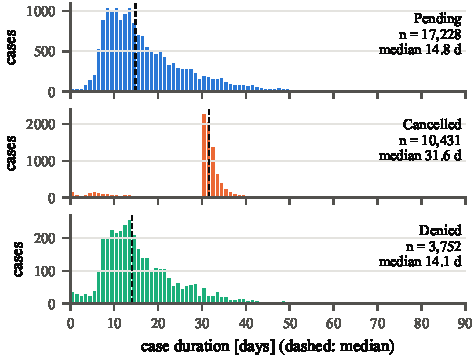
\includegraphics[width=0.6\textwidth]{figures/duration_by_outcome.pdf}
  \caption{Case duration by outcome (modelling log). Cancelled applications
  cluster at 30--32 days, the automatic cancellation when the customer does
  not reply; approved and denied applications end after about two weeks.}
  \label{fig:duration}
\end{figure}

\begin{figure}[h]
  \centering
  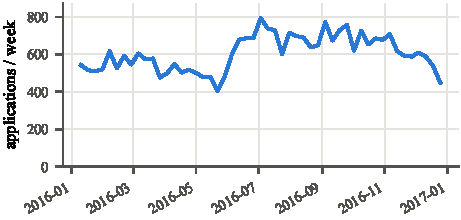
\includegraphics[width=0.6\textwidth]{figures/weekly_arrivals.pdf}
  \caption{New applications per week in 2016. The volume rises from about 500
  to about 700 per week in June 2016.}
  \label{fig:arrivals}
\end{figure}

\clearpage
\subsection{Process Model Creation and Validation}

\begin{table}[h]
  \caption{Iteration log: one row per model version (data change, then
  rediscovery). Fitting cases from alignments, precision (ETC, token-based
  replay with the not-in-model rule) and generalization (alignments), all on
  the full modelling log (31,411 cases). Logs: A = A\_ and O\_ events at
  \texttt{complete}; B1 = A plus W\_ \texttt{start} events; B1c = B1 without
  O\_Created, O\_Accepted and O\_Refused; C = all activities at
  \texttt{complete}. Versions: It0 is the IMf base model; from It1 on, the two
  O\_Sent labels are merged; It2 adds the work items (log B1) at four noise
  thresholds; It3 additionally collapses direct repetitions of the same
  activity; It4--It6 and It8 discover with IM on the most frequent variants
  covering the given share of cases (cov.), on logs A, B1, B1c and C; It7
  repeats It6\_c75 without the rare work items W\_Assess potential fraud,
  W\_Shortened completion and W\_Personal Loan collection.
  $^\dagger$ final model (precision with alignments: 0.701).}
  \centering\small
  \begin{tabular}{lllrrrrr}
    \toprule
    \textbf{Version} & \textbf{Log} & \textbf{Discovery} & \textbf{Fit.\ [\%]} &
    \textbf{Prec.} & \textbf{Gen.} & \textbf{CNC} & \textbf{Size} \\
    \midrule
It0 & A & IMf 0.10 & 88.7 & 0.590 & 0.989 & 1.23 & 163 \\
It1 & A & IMf 0.10 & 93.0 & 0.589 & 0.989 & 1.23 & 163 \\
It2\_05 & B1 & IMf 0.05 & 96.2 & 0.407 & 0.879 & 1.26 & 305 \\
It2\_10 & B1 & IMf 0.10 & 85.9 & 0.432 & 0.903 & 1.26 & 291 \\
It2\_15 & B1 & IMf 0.15 & 58.5 & 0.528 & 0.897 & 1.25 & 274 \\
It2\_20 & B1 & IMf 0.20 & 58.5 & 0.505 & 0.897 & 1.25 & 274 \\
It3 & B1 & IMf 0.10 & 85.9 & 0.439 & 0.948 & 1.27 & 218 \\
It4\_c60 & A & IM, 60\,\% cov. & 72.5 & 0.862 & 0.991 & 1.17 & 104 \\
It4\_c65 & A & IM, 65\,\% cov. & 75.5 & 0.710 & 0.991 & 1.18 & 122 \\
It4\_c70 & A & IM, 70\,\% cov. & 86.4 & 0.706 & 0.992 & 1.20 & 132 \\
It4\_c72.5 & A & IM, 72.5\,\% cov. & 86.4 & 0.706 & 0.992 & 1.20 & 132 \\
It4\_c75 & A & IM, 75\,\% cov. & 88.4 & 0.706 & 0.991 & 1.20 & 143 \\
It4\_c80 & A & IM, 80\,\% cov. & 92.0 & 0.675 & 0.991 & 1.20 & 143 \\
It4\_c90 & A & IM, 90\,\% cov. & 99.4 & 0.585 & 0.983 & 1.23 & 185 \\
It5\_c60 & B1 & IM, 60\,\% cov. & 72.8 & 0.659 & 0.991 & 1.19 & 158 \\
It5\_c65 & B1 & IM, 65\,\% cov. & 83.1 & 0.657 & 0.991 & 1.21 & 168 \\
It5\_c70 & B1 & IM, 70\,\% cov. & 85.0 & 0.657 & 0.991 & 1.21 & 179 \\
It5\_c72.5 & B1 & IM, 72.5\,\% cov. & 88.4 & 0.613 & 0.991 & 1.21 & 179 \\
It5\_c75 & B1 & IM, 75\,\% cov. & 89.4 & 0.710 & 0.991 & 1.22 & 182 \\
It5\_c80 & B1 & IM, 80\,\% cov. & 97.2 & 0.514 & 0.988 & 1.23 & 203 \\
It5\_c90 & B1 & IM, 90\,\% cov. & 99.9 & 0.290 & 0.977 & 1.26 & 265 \\
It6\_c60 & B1c & IM, 60\,\% cov. & 74.6 & 0.680 & 0.991 & 1.21 & 146 \\
It6\_c65 & B1c & IM, 65\,\% cov. & 85.0 & 0.676 & 0.992 & 1.22 & 160 \\
It6\_c70 & B1c & IM, 70\,\% cov. & 85.0 & 0.676 & 0.992 & 1.22 & 160 \\
It6\_c72.5 & B1c & IM, 72.5\,\% cov. & 88.4 & 0.625 & 0.992 & 1.22 & 160 \\
It6\_c75$^\dagger$ & B1c & IM, 75\,\% cov. & 89.4 & 0.700 & 0.991 & 1.23 & 163 \\
It6\_c80 & B1c & IM, 80\,\% cov. & 97.3 & 0.514 & 0.988 & 1.25 & 180 \\
It6\_c90 & B1c & IM, 90\,\% cov. & 99.9 & 0.334 & 0.975 & 1.29 & 284 \\
It7 & B1c & IM, 75\,\% cov. & 89.6 & 0.631 & 0.991 & 1.24 & 170 \\
It8\_c60 & C & IM, 60\,\% cov. & 82.1 & 0.594 & 0.991 & 1.21 & 197 \\
It8\_c70 & C & IM, 70\,\% cov. & 91.3 & 0.455 & 0.989 & 1.25 & 205 \\
    \bottomrule
  \end{tabular}
  \label{tab:iterations}
\end{table}

\begin{figure}[h]
  \centering
  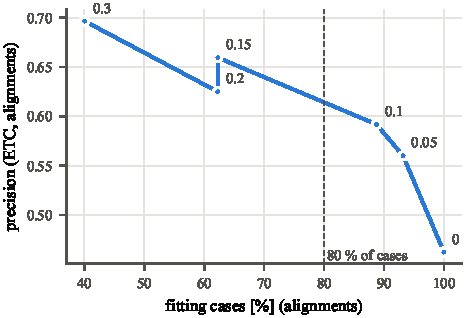
\includegraphics[width=0.5\textwidth]{figures/imf_sweep.pdf}
  \caption{Noise threshold sweep of the Inductive Miner infrequent on the
  A\_/O\_ events (labels: noise threshold). From 0.15 on, IMf filters the loop
  around the offer block, and the fitting cases drop from 88.7\,\% to
  62.3\,\%.}
  \label{fig:imfsweep}
\end{figure}

\begin{figure}[h]
  \centering
  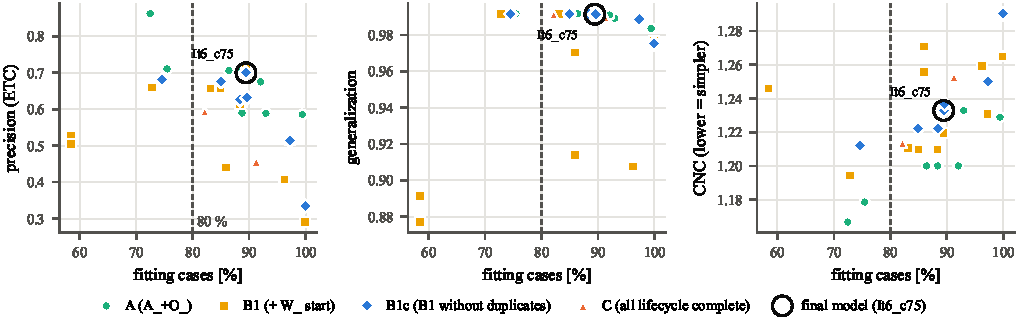
\includegraphics[width=\textwidth]{figures/tradeoff_panels.pdf}
  \caption{Trade-off between fitting cases and precision, generalization and
  simplicity (CNC) for every version in Table~\ref{tab:iterations}; the final
  model is ringed. The dashed line marks the 80\,\% threshold.}
  \label{fig:tradeoff}
\end{figure}

\begin{figure}[h]
  \centering
  \begin{minipage}[t]{0.48\textwidth}
    \centering
    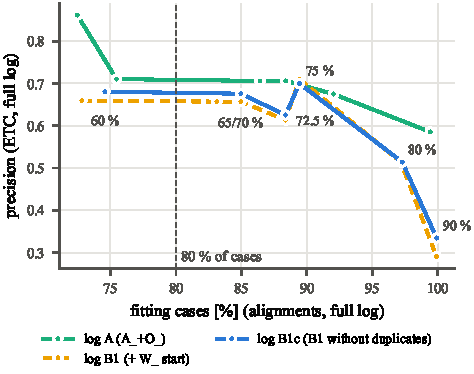
\includegraphics[width=\linewidth]{figures/coverage_tradeoff.pdf}
    \caption{Effect of the variant coverage used for discovery (labels) on
    fitting cases and precision, per log version.}
    \label{fig:coveragetradeoff}
  \end{minipage}\hfill
  \begin{minipage}[t]{0.48\textwidth}
    \centering
    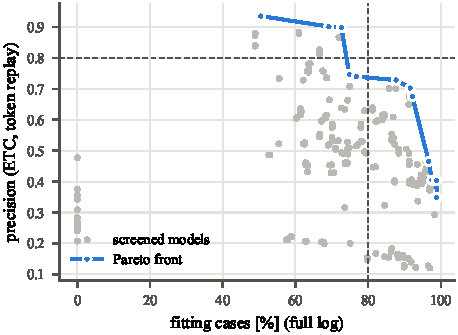
\includegraphics[width=\linewidth]{figures/explore_w_complete_pareto.pdf}
    \caption{360 screened models with W\_ items at lifecycle \texttt{complete}
    (logs C and variants, several miners). No model reaches a precision of 0.8
    with at least 80\,\% fitting cases.}
    \label{fig:pareto}
  \end{minipage}
\end{figure}

\begin{figure}[h]
  \centering
  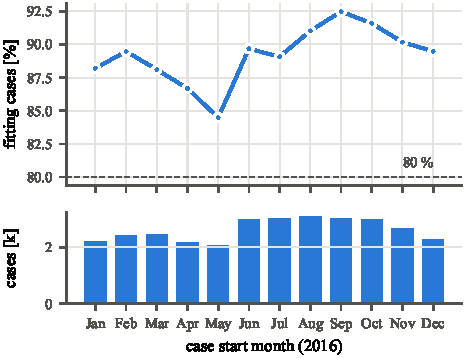
\includegraphics[width=0.6\textwidth]{figures/fitting_by_month.pdf}
  \caption{Fitting cases of the final model by case start month (top) and
  number of cases per month (bottom).}
  \label{fig:monthly}
\end{figure}

\clearpage
\subsection{Discovered and Final Models}

\begin{figure}[h!]
  \centering
  
\includegraphics[width=\textwidth]{figures/IM.pdf}
  \caption{Petri net discovered with the Inductive Miner on the A\_/O\_ events
  (log A). With 73\,\% silent transitions and loops that allow almost any
  order, it is close to a flower model: it replays every case but has a
  precision of only 0.46 and an extended cyclomatic complexity of 77,728.}
  \label{fig:im}
\end{figure}

\begin{figure}[h!]
  \centering
  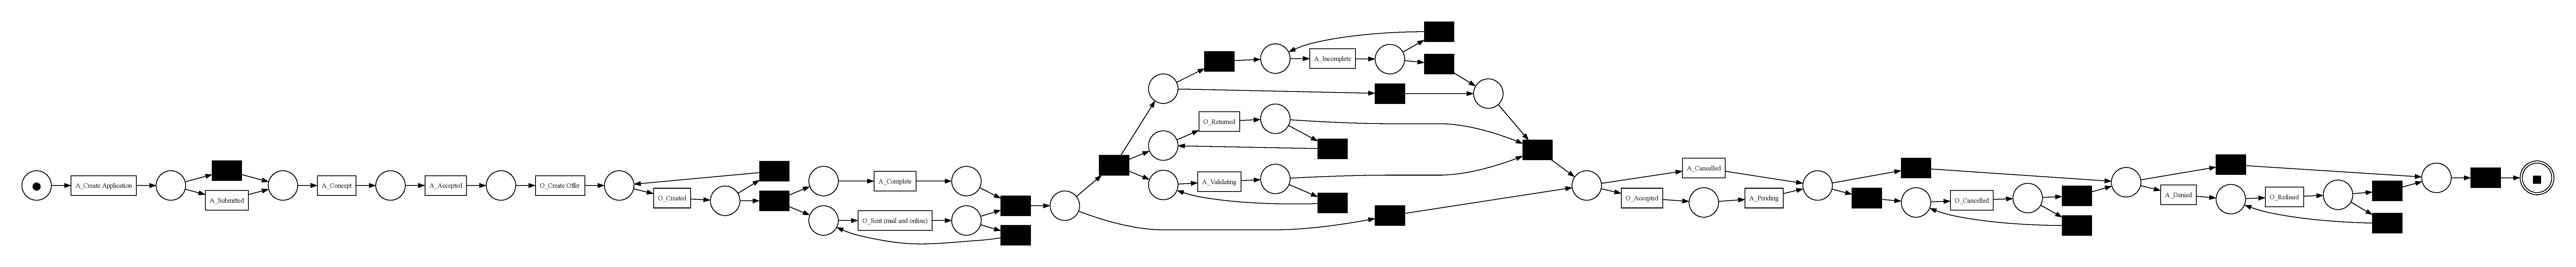
\includegraphics[width=\textwidth]{figures/IMf.pdf}
  \caption{Petri net discovered with the Inductive Miner infrequent (noise
  threshold 0.2) on the A\_/O\_ events (log A).}
  \label{fig:imf}
\end{figure}

\begin{figure}[h!]
  \centering
  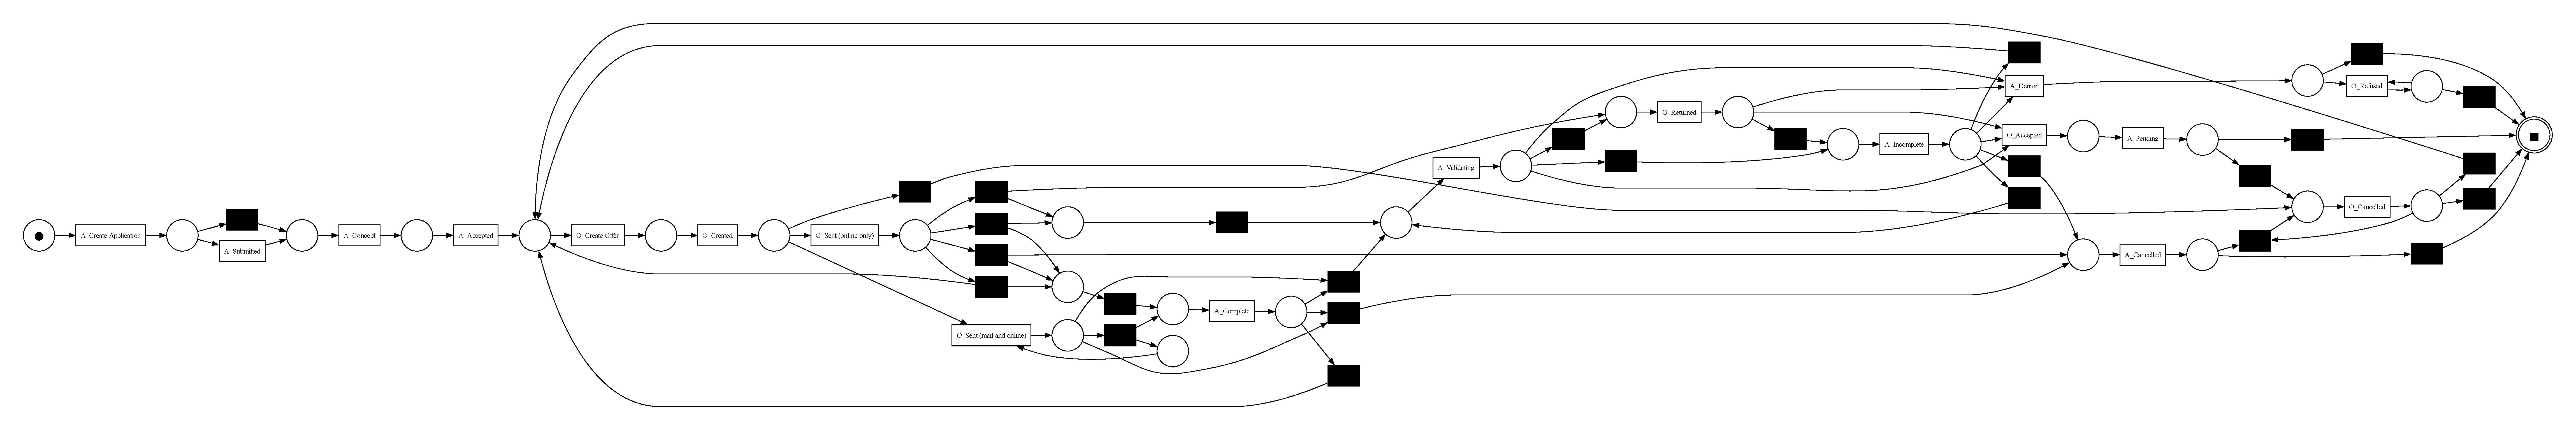
\includegraphics[width=\textwidth]{figures/HM.pdf}
  \caption{Petri net discovered with the Heuristics Miner (PM4Py defaults) on
  the A\_/O\_ events (log A).}
  \label{fig:hm}
\end{figure}

\begin{figure}[h!]
  \centering
  
\includegraphics[width=\textwidth]{figures/final.pdf}
  \caption{Final Petri net (It6\_c75): Inductive Miner on the variants
  covering 75\,\% of the cases of the modelling log.}
  \label{fig:finalpn}
\end{figure}

\begin{figure}[h!]
  \centering
  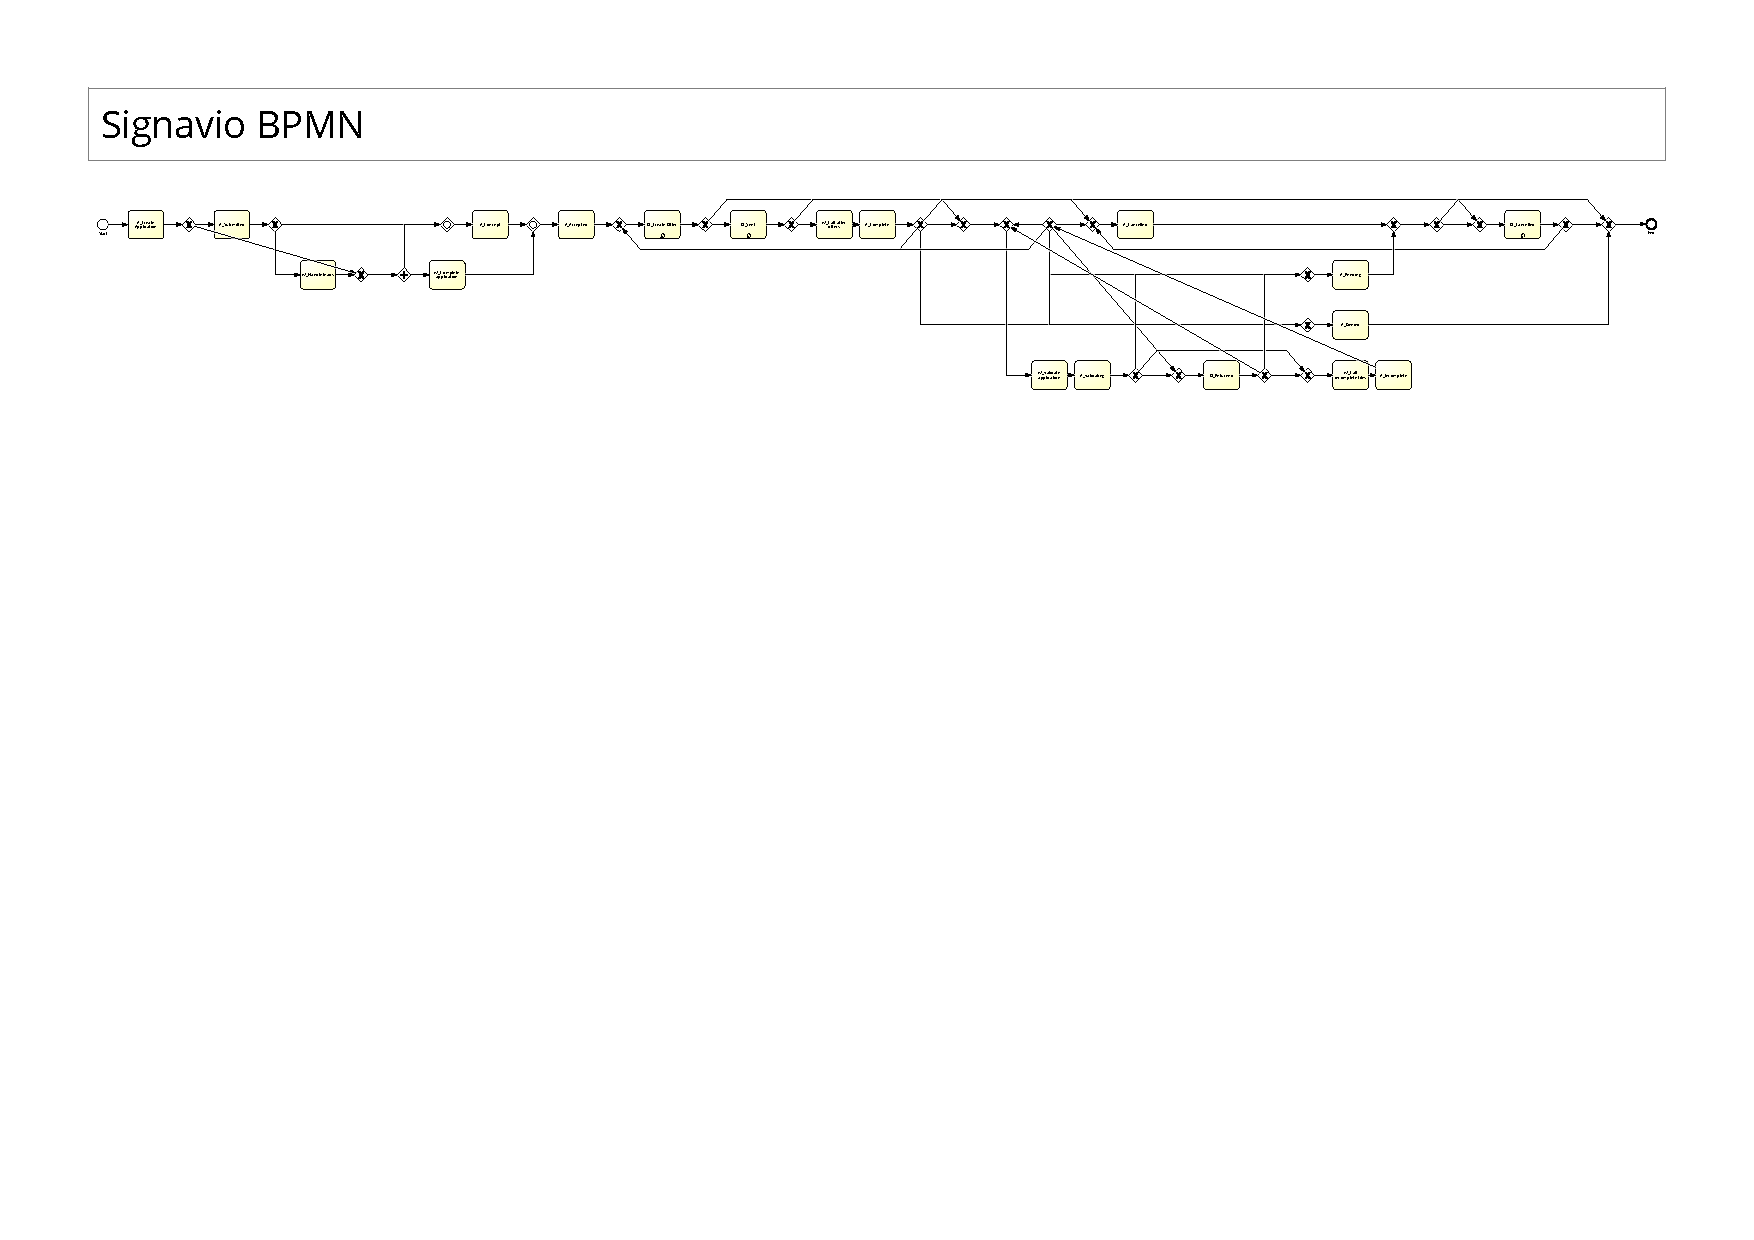
\includegraphics[width=\textwidth,trim=44 406 45 94,clip]{figures/signavio_bpmn.pdf}
  \caption{BPMN generated by SAP Signavio Process Intelligence (Variant
  Explorer, ``Generate BPMN'') from the 92 most frequent variants, the same
  input as the final model.}
  \label{fig:signaviogen}
\end{figure}

\clearpage
\subsection{Decision Mining}

\begin{table}[h]
  \caption{Decision points of the final model with their observed branching
  probabilities (share of visits). Types: XOR = exclusive choice, loop =
  loop decision repeating a block, self = self-loop. Mined rules for D6, D9
  and D10 in Section~\ref{sec:dm}; for all other points, the probabilities are
  the simulation input.}
  \centering\small
  \begin{tabular}{llll}
    \toprule
    \textbf{ID} & \textbf{Type} & \textbf{Decision} & \textbf{Branches} \\
    \midrule
    D1  & XOR  & O\_Sent after an offer           & sent 89.5\,\%, skipped 10.5\,\% \\
    D2  & loop & further round of offers          & repeat 26.5\,\%, exit 73.5\,\% \\
    D3  & self & O\_Sent repeated                 & repeat 7.7\,\%, continue 92.3\,\% \\
    D4  & XOR  & W\_Call incomplete files         & call 59.2\,\%, no call 40.8\,\% \\
    D5  & loop & further validation round         & repeat 39.4\,\%, exit 60.6\,\% \\
    D6  & XOR  & W\_Call after offers (rule)      & call 81.8\,\%, no call 18.2\,\% \\
    D7  & XOR  & offer returned by the customer   & returned 61.3\,\%, not returned 38.7\,\% \\
    D8  & XOR  & W\_Complete application          & started 93.9\,\%, skipped 6.1\,\% \\
    D9  & XOR  & outcome (rule)                   & Pending 54.9\,\%, Cancelled 33.2\,\%, Denied 11.9\,\% \\
    D10 & XOR  & channel (rule)                   & online 64.8\,\%, bank 35.2\,\% \\
    D11 & XOR  & cancellation events (bookkeeping) & cancelled 53.8\,\%, end 46.2\,\% \\
    D12 & XOR  & W\_Handle leads (manual check)   & manual 17.8\,\%, automatic 82.2\,\% \\
    D13 & self & further O\_Cancelled (bookkeeping) & repeat 22.5\,\%, end 77.5\,\% \\
    D14 & XOR  & A\_Cancelled (bookkeeping)       & A\_Cancelled 70.1\,\%, end 29.9\,\% \\
    \bottomrule
  \end{tabular}
  \label{tab:dpoints}
\end{table}

\begin{figure}[h]
  \centering
  \begin{minipage}[t]{0.48\textwidth}
    \centering
    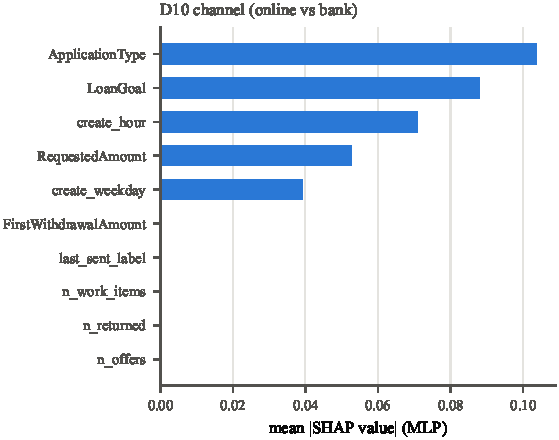
\includegraphics[width=\linewidth]{figures/shap_D10.pdf}\\
    {\small (a) Channel (D10)}
  \end{minipage}\hfill
  \begin{minipage}[t]{0.48\textwidth}
    \centering
    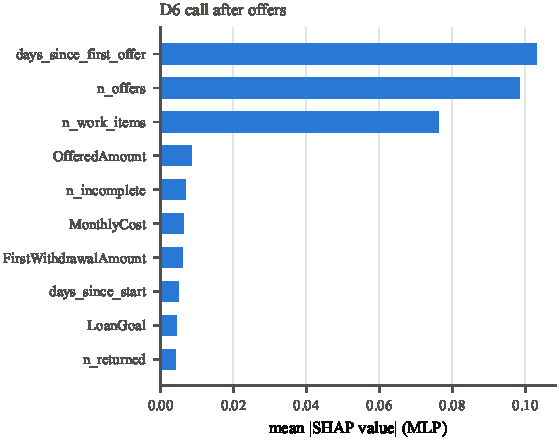
\includegraphics[width=\linewidth]{figures/shap_D6.pdf}\\
    {\small (b) Call after offers (D6)}
  \end{minipage}\\[8pt]
  \begin{minipage}[t]{0.48\textwidth}
    \centering
    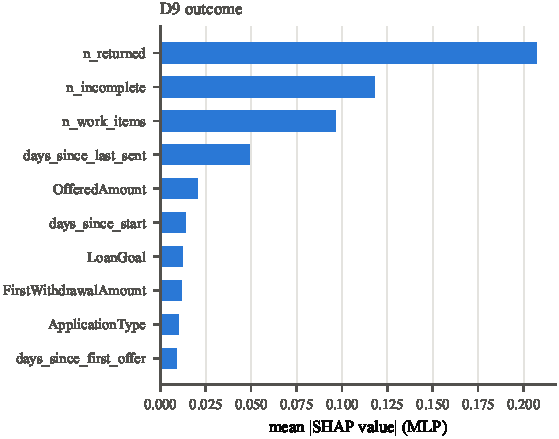
\includegraphics[width=\linewidth]{figures/shap_D9.pdf}\\
    {\small (c) Outcome (D9)}
  \end{minipage}\hfill
  \begin{minipage}[t]{0.48\textwidth}
    \centering
    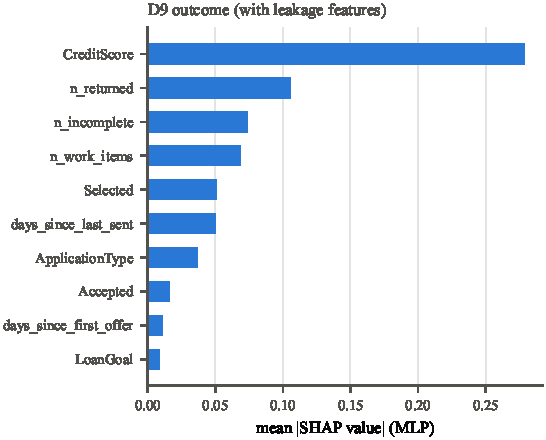
\includegraphics[width=\linewidth]{figures/shap_D9_leakage.pdf}\\
    {\small (d) Outcome with CreditScore, Selected and Accepted}
  \end{minipage}
  \caption{Mean absolute SHAP values of the neural network on the test cases
  for the three decisions with good rules (a--c). The top features match the
  splits of the decision trees. With the leaking features (d), CreditScore
  dominates.}
  \label{fig:shap}
\end{figure}

\clearpage
\subsection{SAP Signavio}\label{sec:app_signavio}

\begin{figure}[h!]
  \centering
  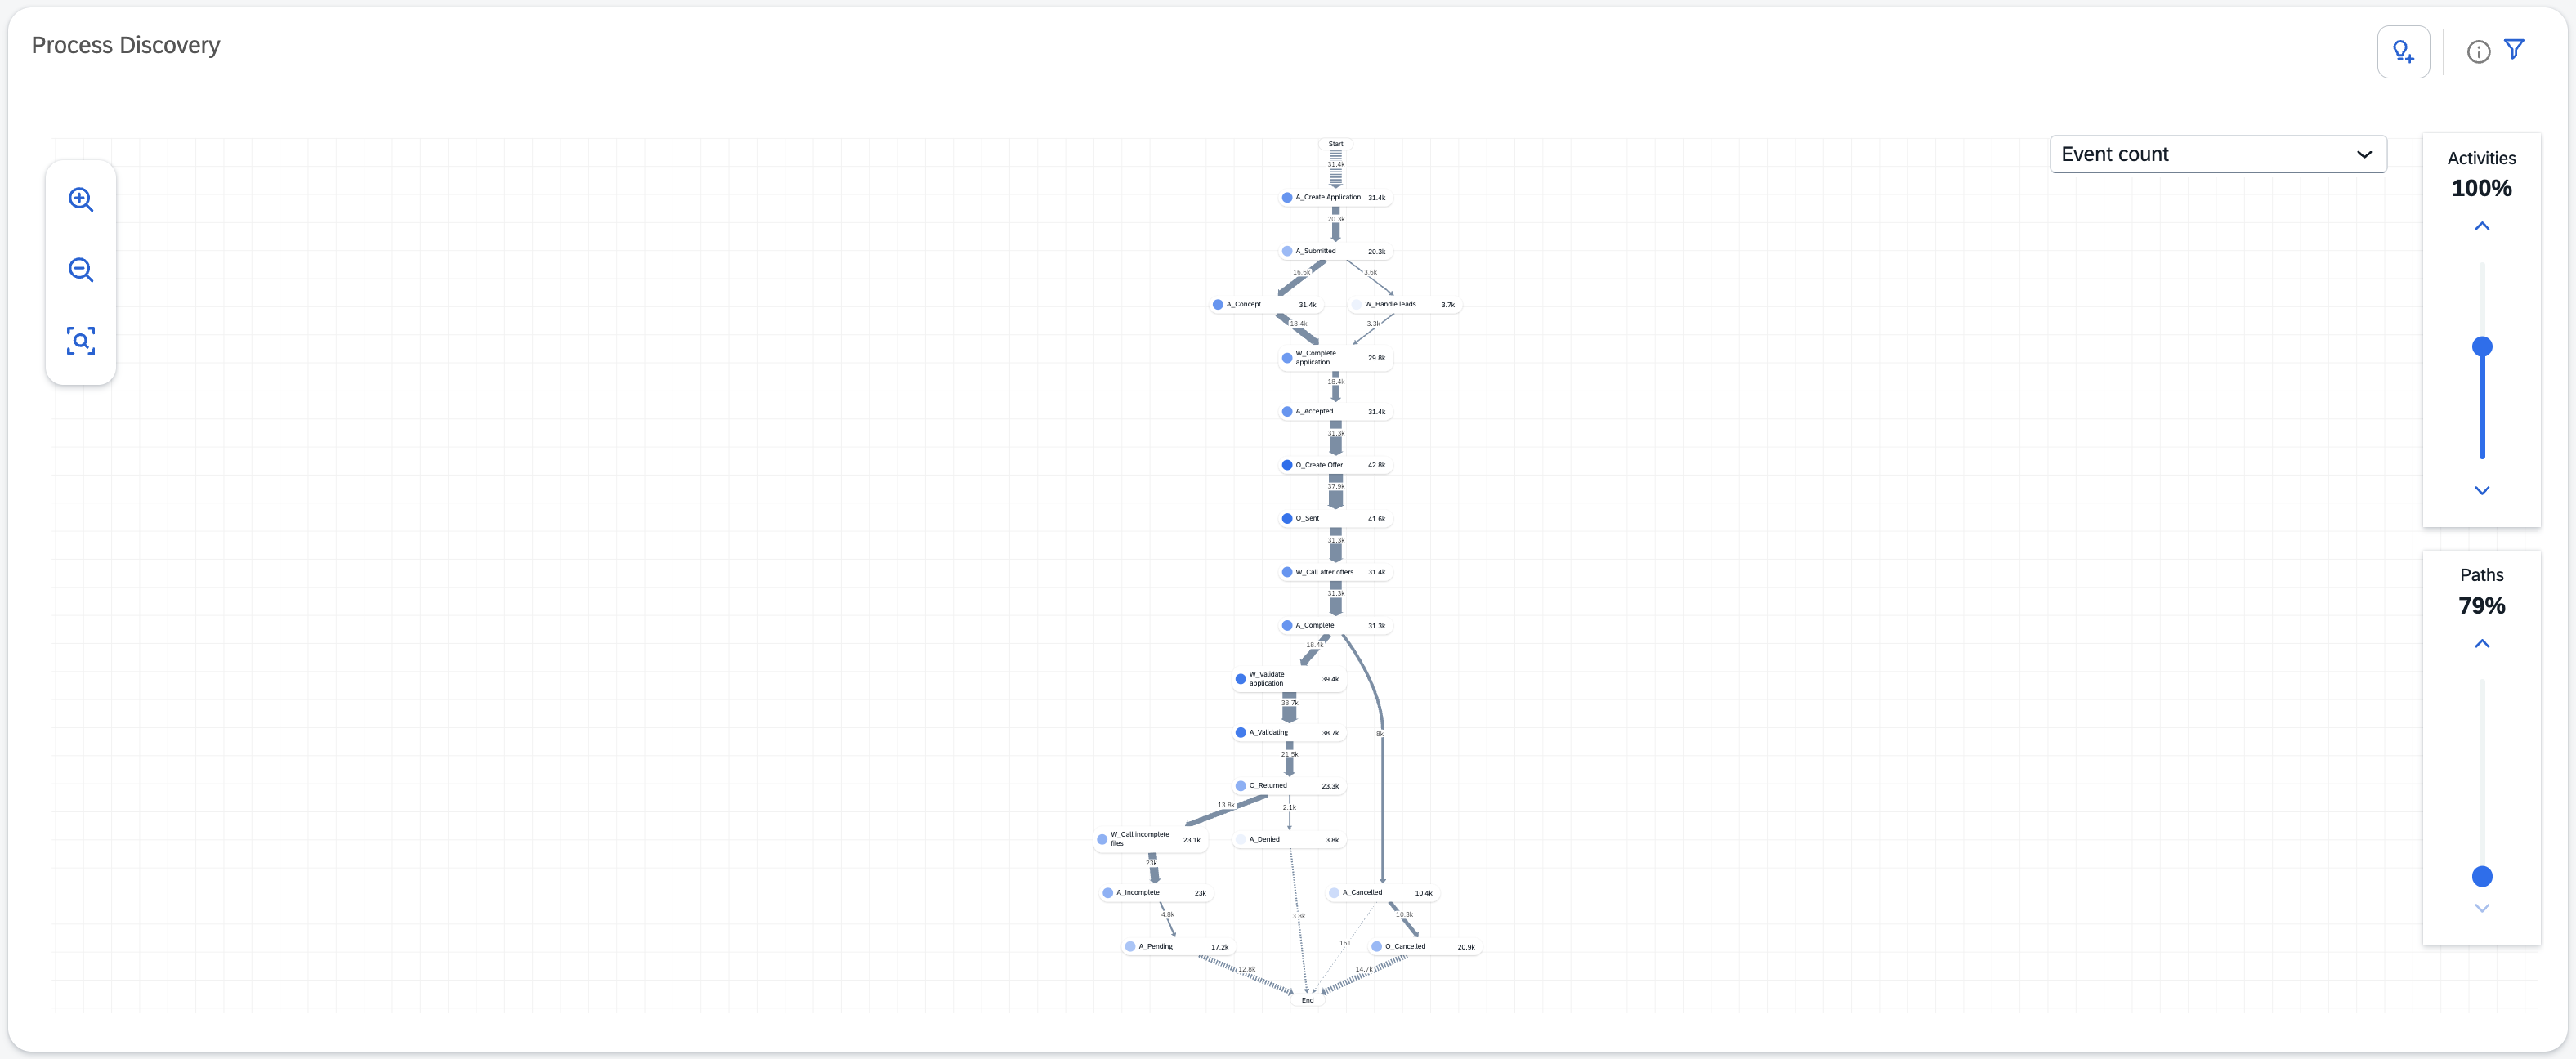
\includegraphics[width=0.75\textwidth]{figures/Process_Discovery.png}
  \caption{Process Intelligence: discovery map of the modelling log (all
  activities, minimum of 79\,\% of the paths).}
  \label{fig:sig_discovery}
\end{figure}

\begin{figure}[h!]
  \centering
  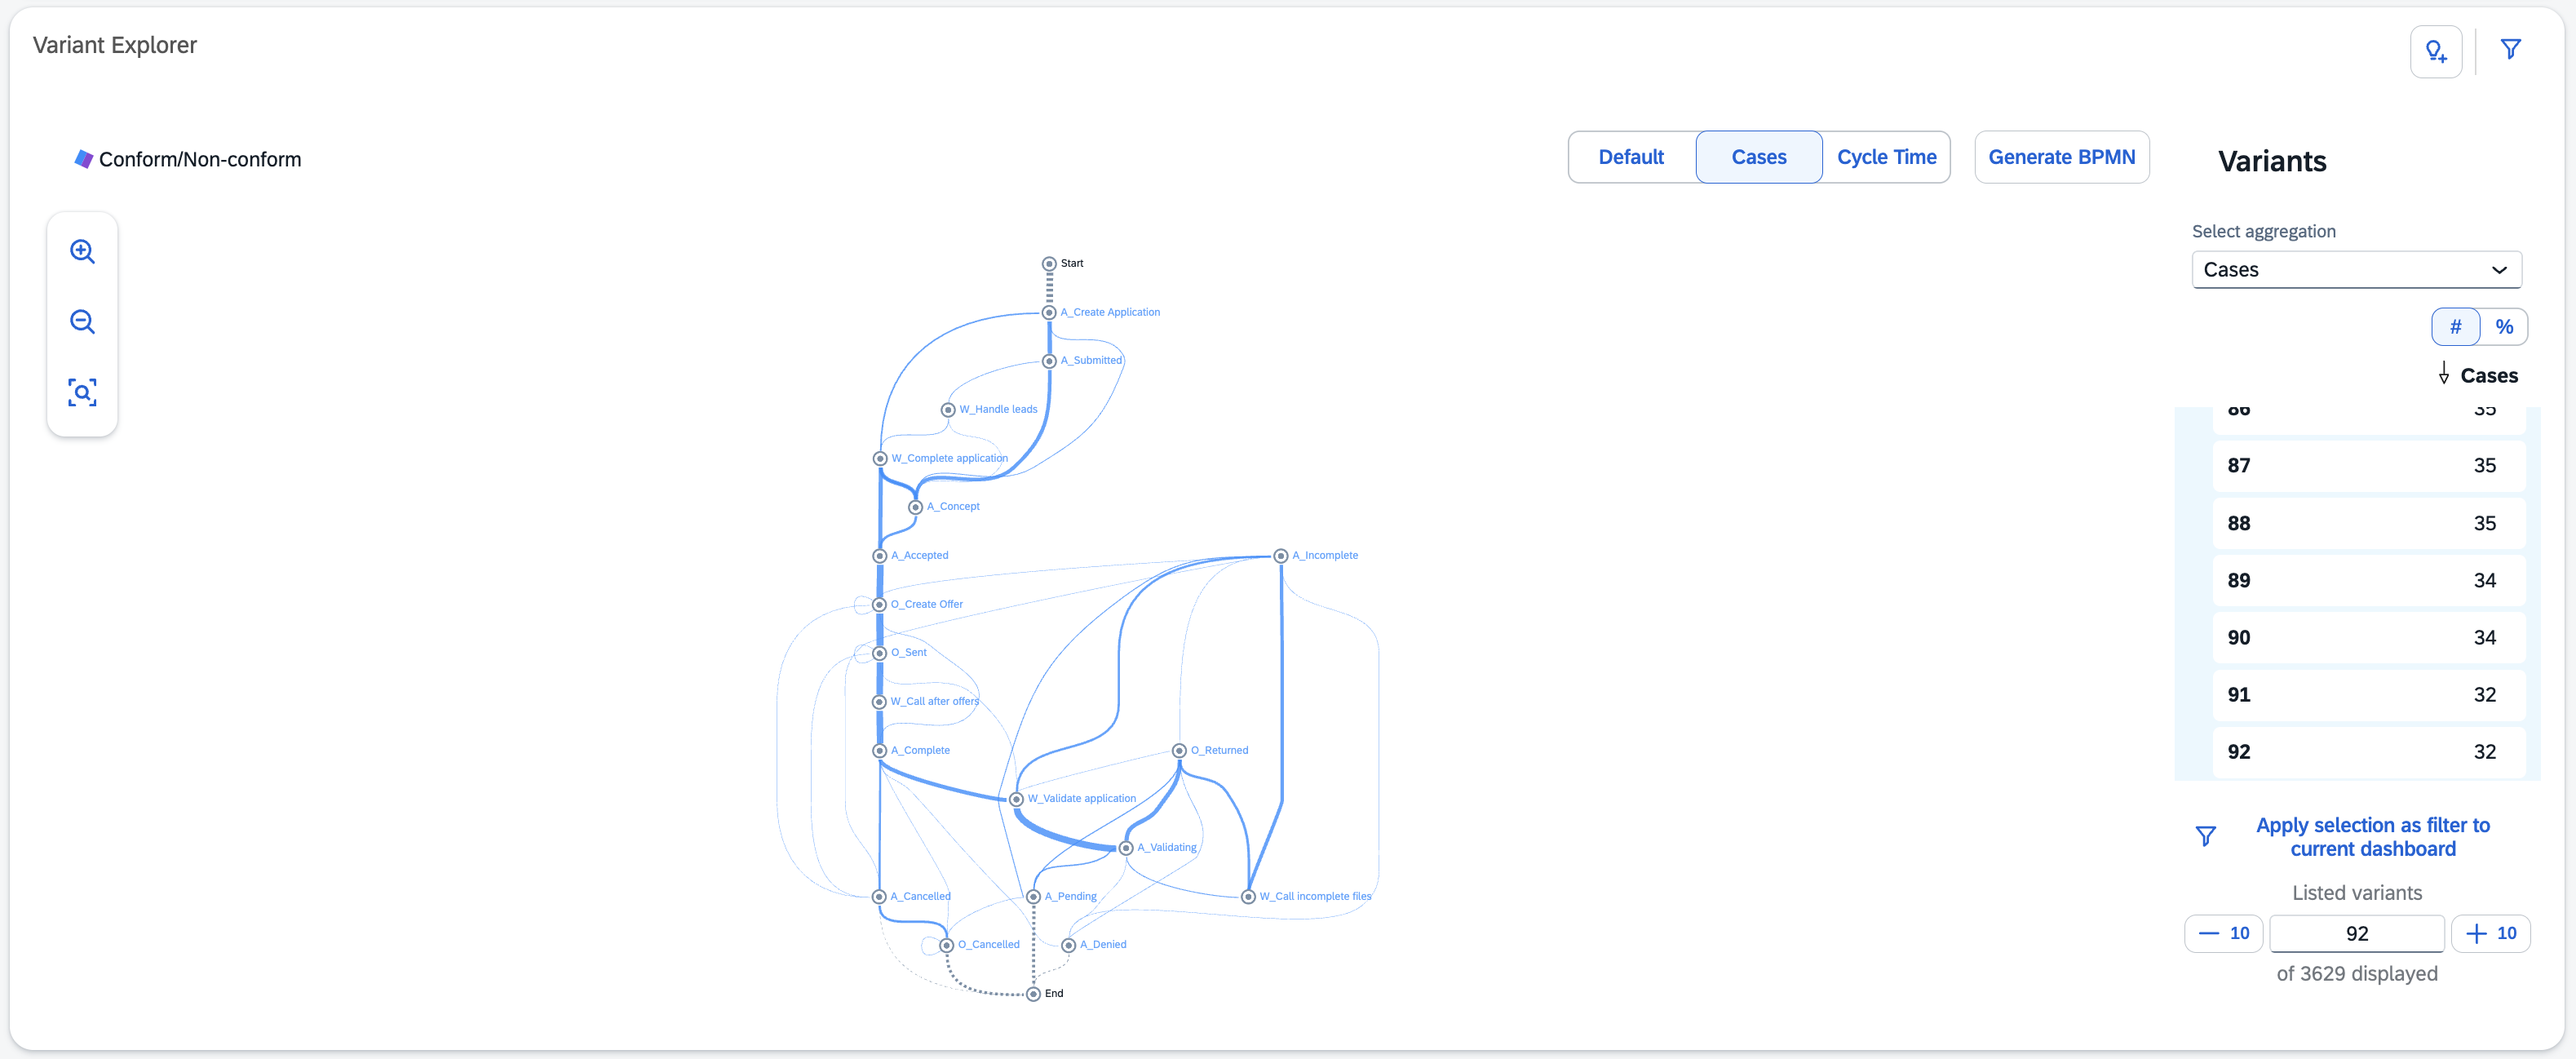
\includegraphics[width=\textwidth]{figures/Variant_Explorer_Top_92.png}
  \caption{Variant Explorer with the 92 most frequent variants (75\,\% of the
  cases), the input for ``Generate BPMN'' (Figure~\ref{fig:signaviogen}).}
  \label{fig:sig_variants}
\end{figure}

\begin{figure}[h!]
  \centering
  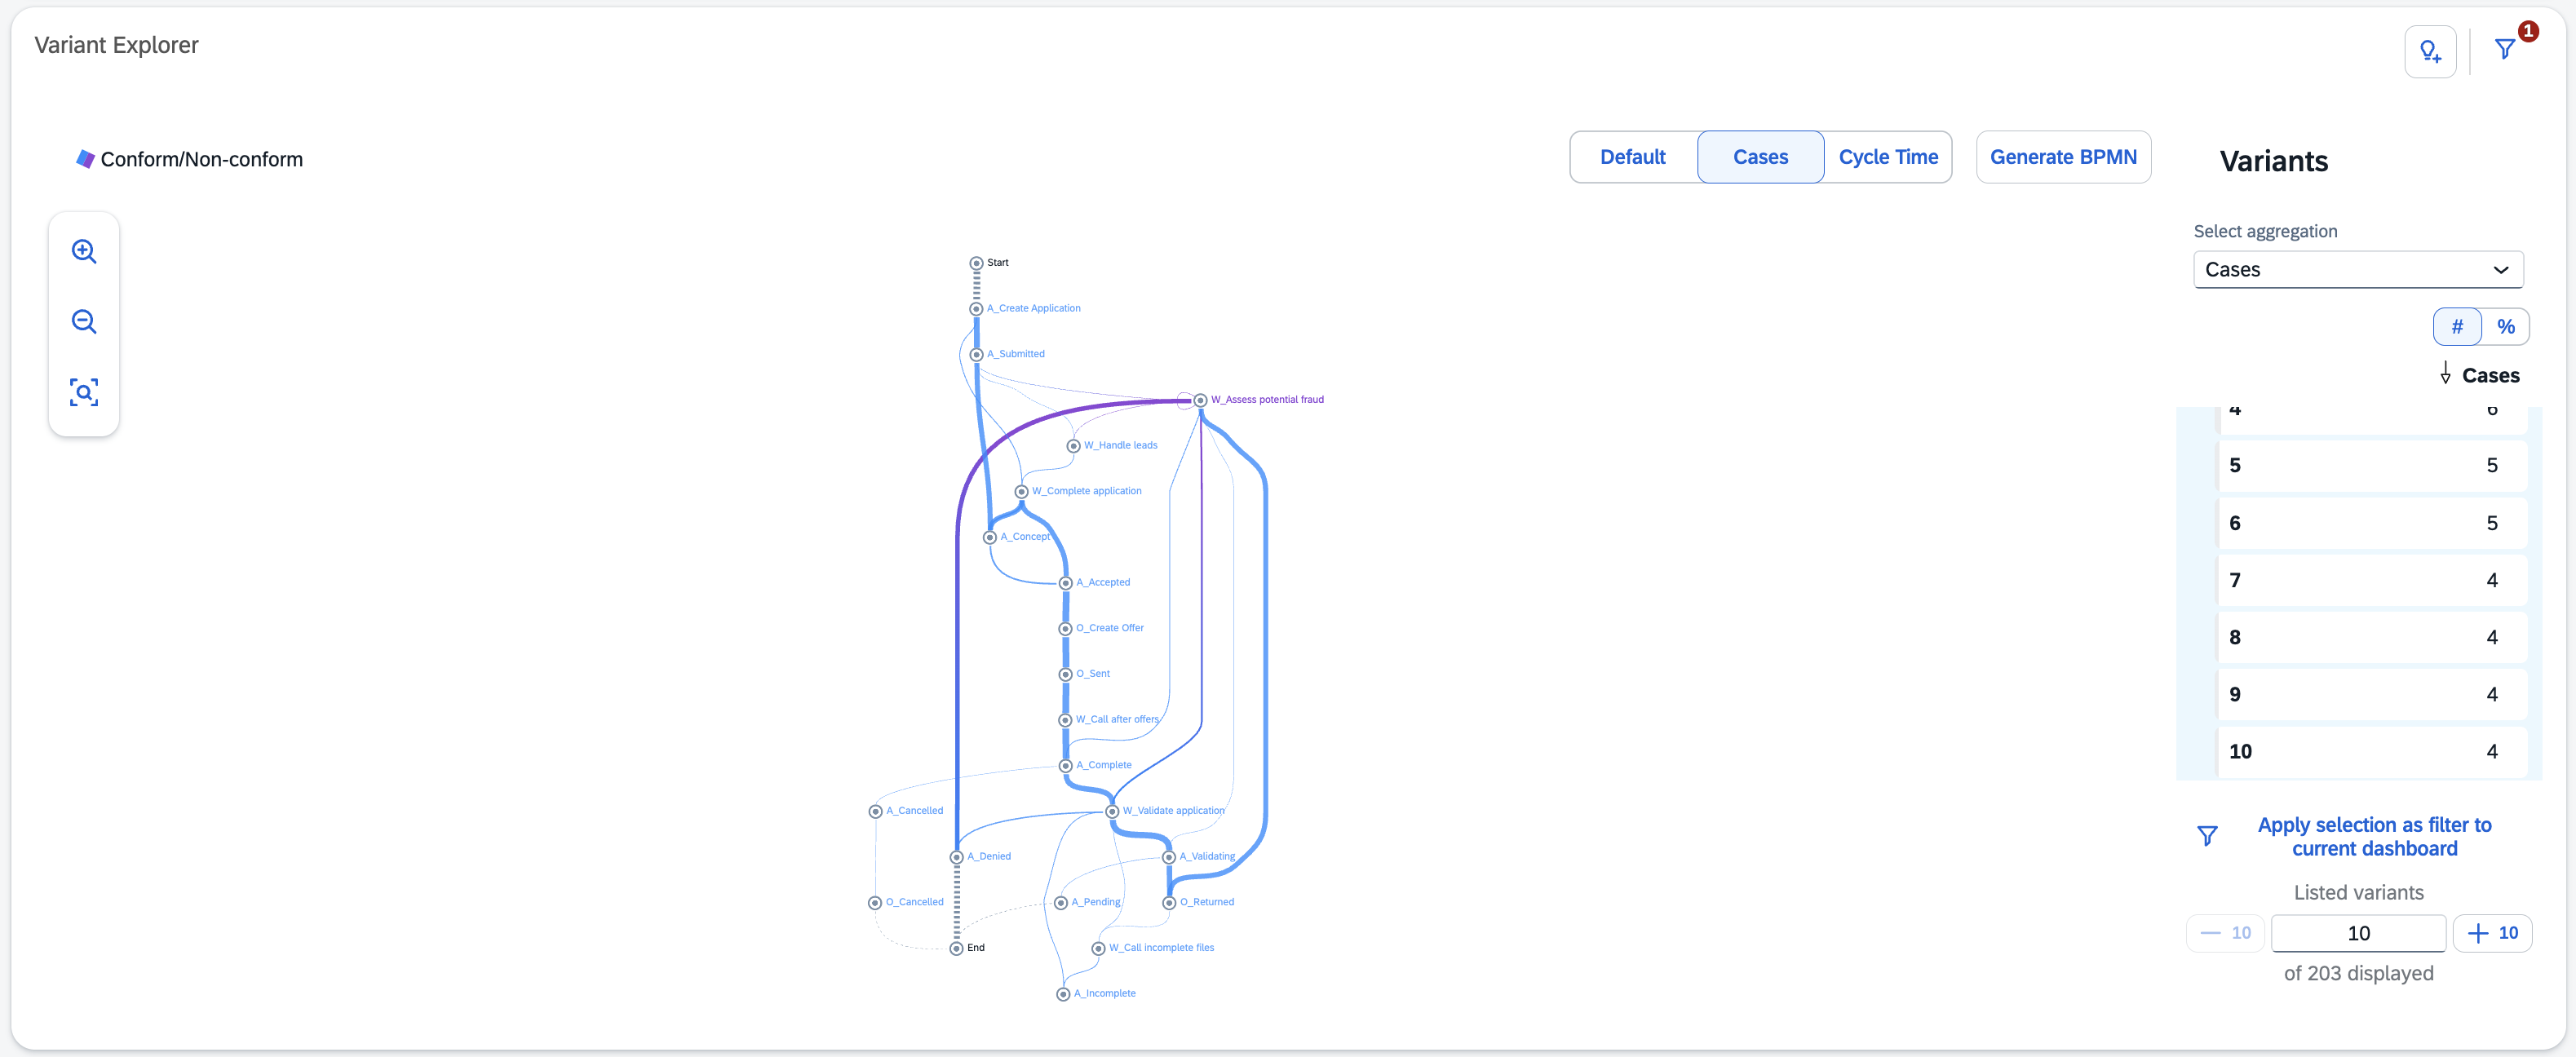
\includegraphics[width=\textwidth]{figures/Conformance_Asses_Fraud_Purple.png}
  \caption{Variant conformance: W\_Assess potential fraud, which is not part of
  the model, is flagged as non-conforming (purple).}
  \label{fig:sig_fraud}
\end{figure}

\begin{figure}[h!]
  \centering
  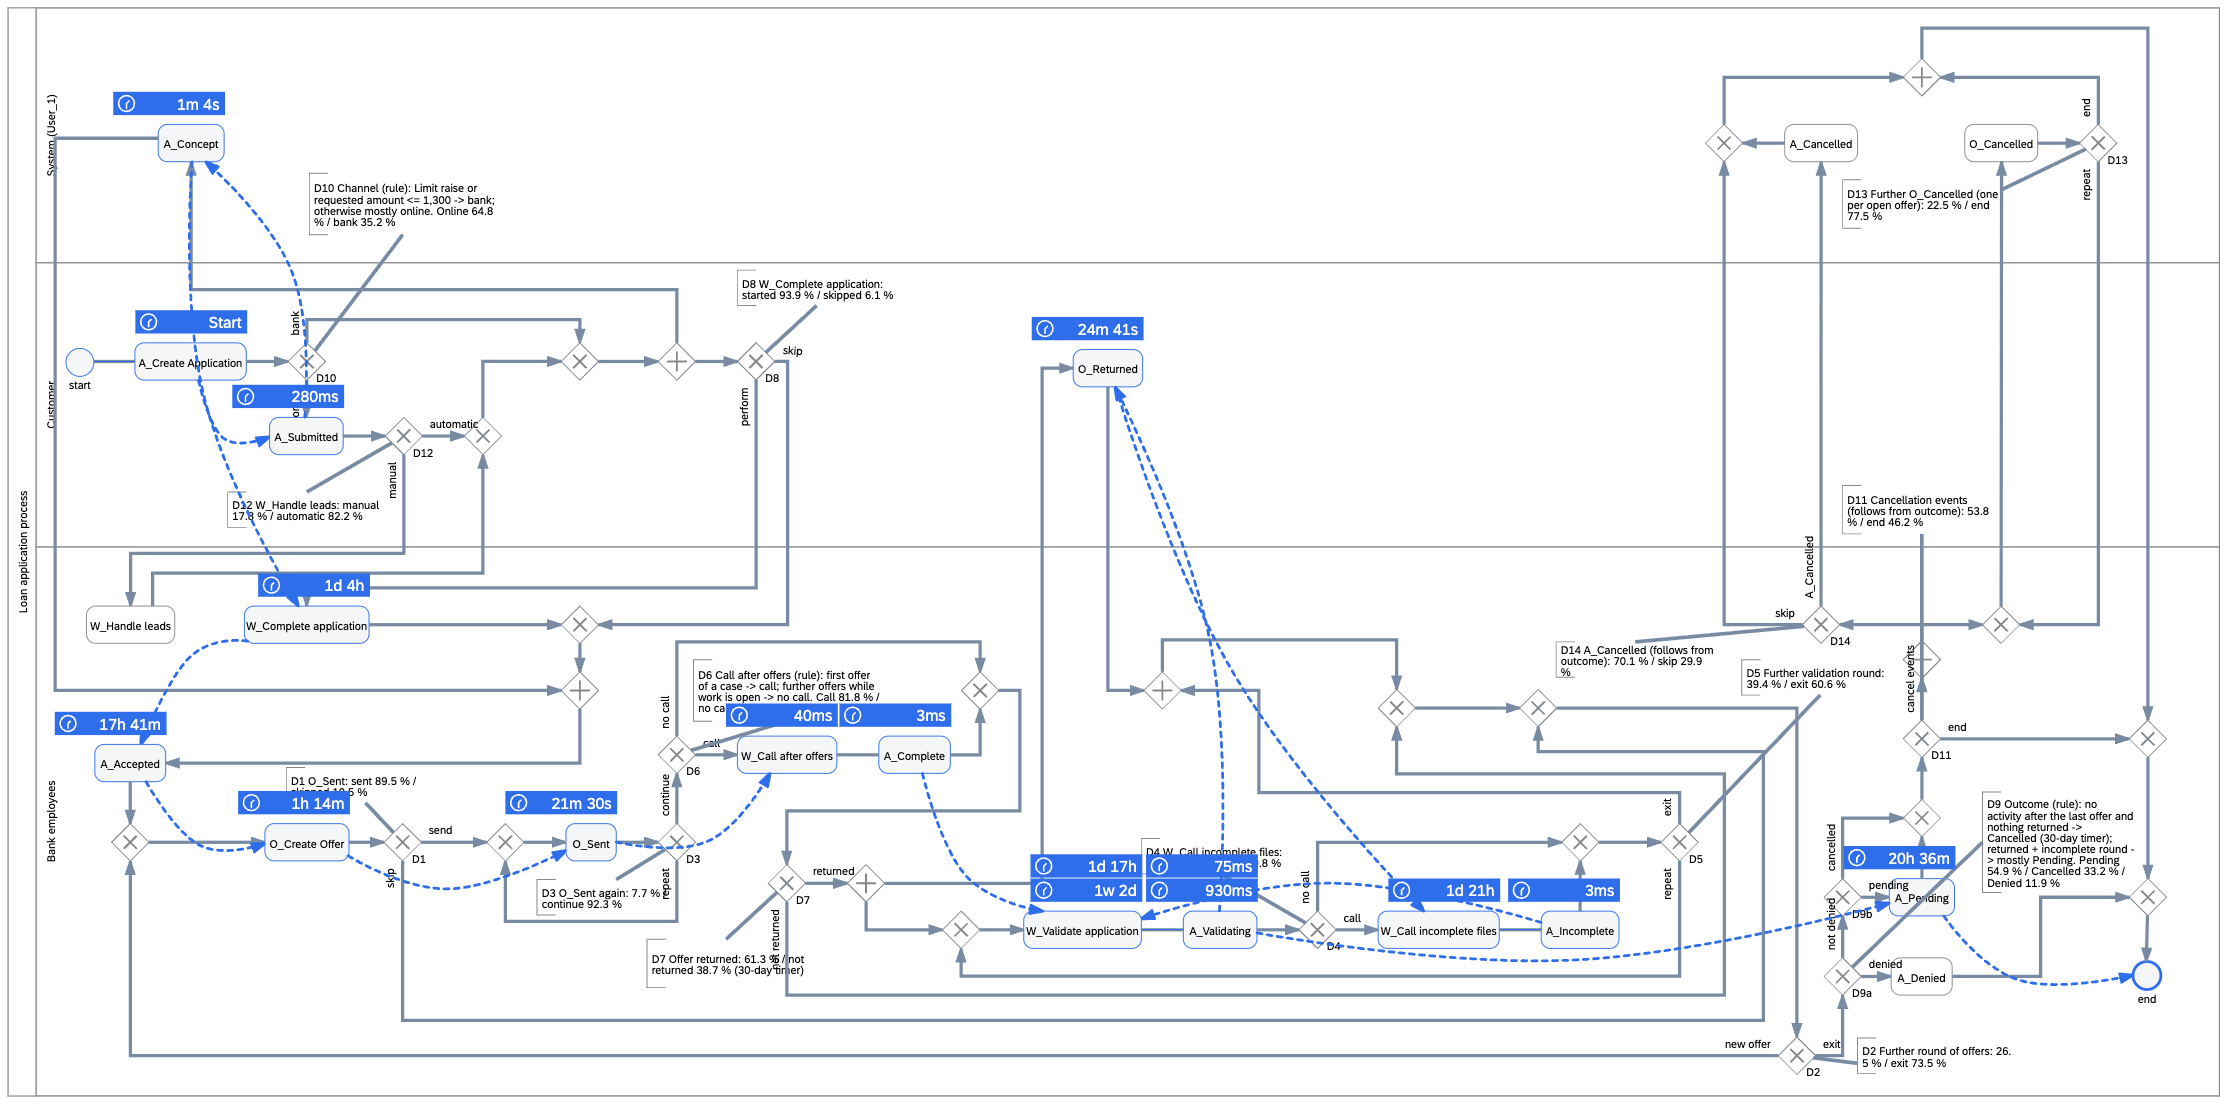
\includegraphics[width=\textwidth]{figures/Conformance_Variant_Overlay.png}
  \caption{Process Conformance widget: a selected variant (dashed path)
  overlaid on the final BPMN with lanes and gateway annotations; the badges
  show the time between consecutive activities, e.g.\ about one day before
  W\_Complete application and up to two weeks within the validation round.}
  \label{fig:sig_overlay}
\end{figure}

\clearpage
\begin{figure}[h!]
  \centering
  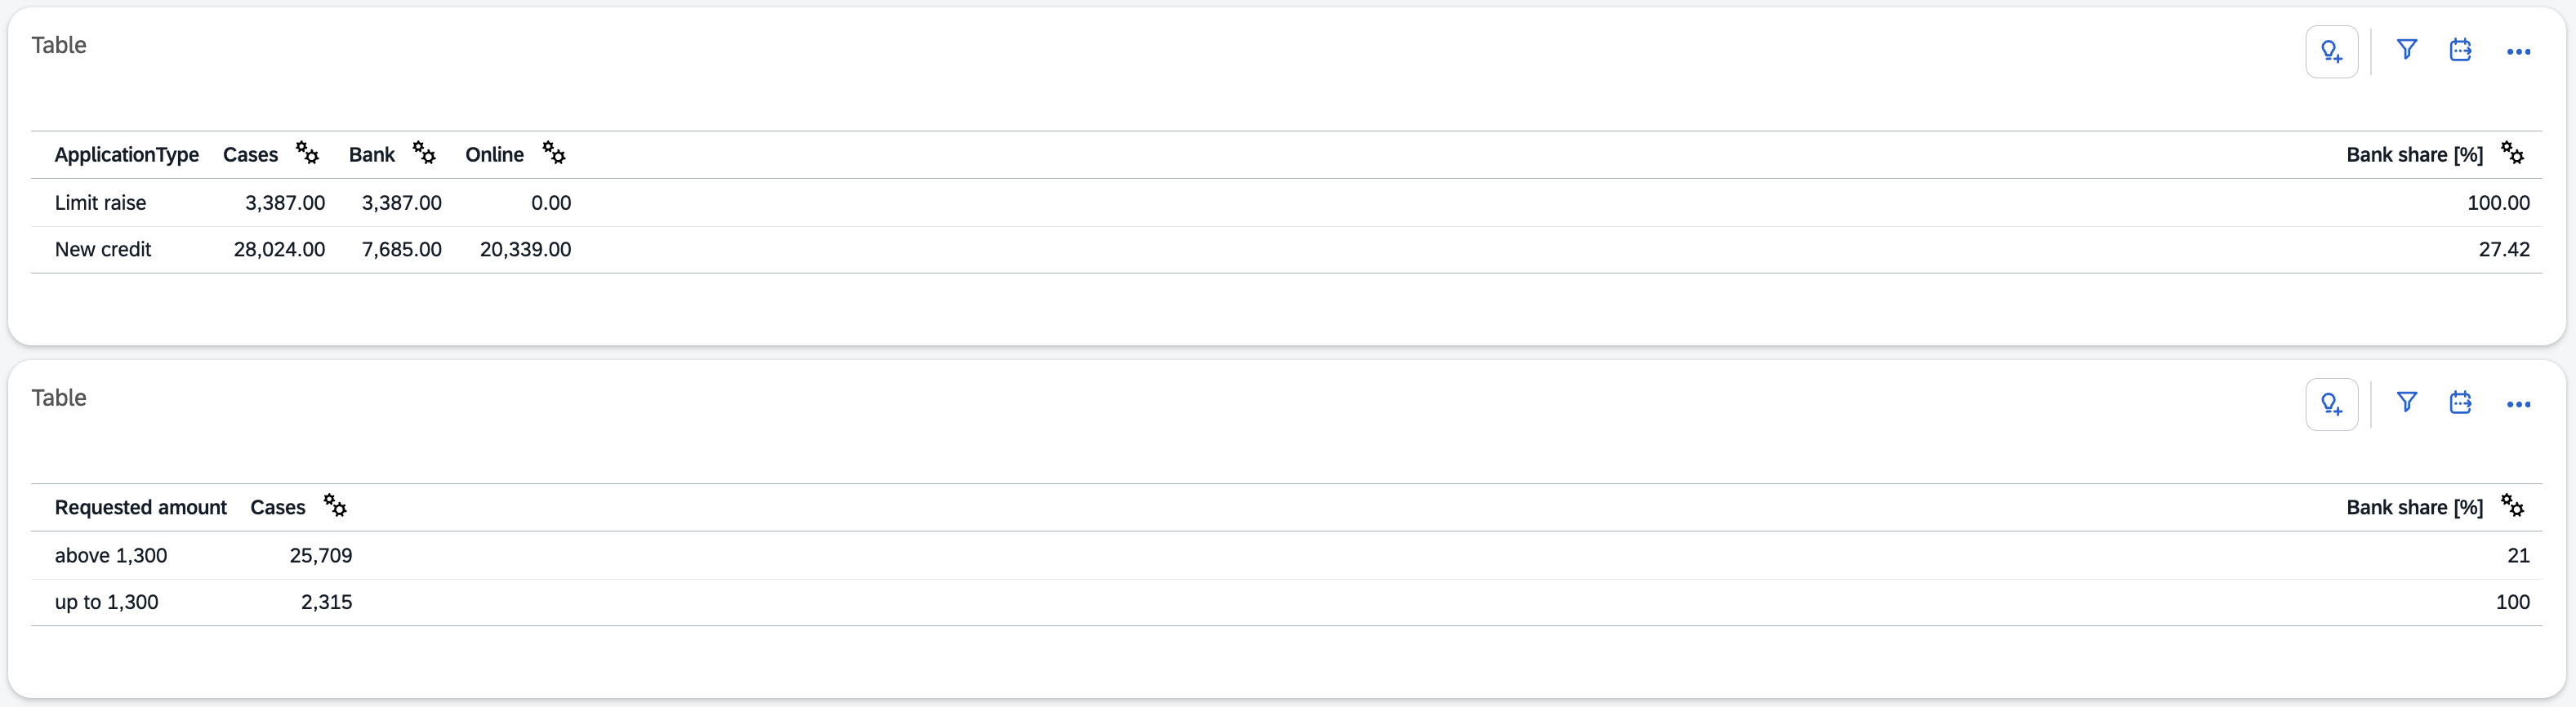
\includegraphics[width=\textwidth]{figures/Query_Tables.png}
  \caption{SIGNAL queries confirming the channel rule (D10): limit raises and
  new credits up to 1,300 are entered by the bank.}
  \label{fig:sig_signal}
\end{figure}

\begin{figure}[h!]
  \centering
  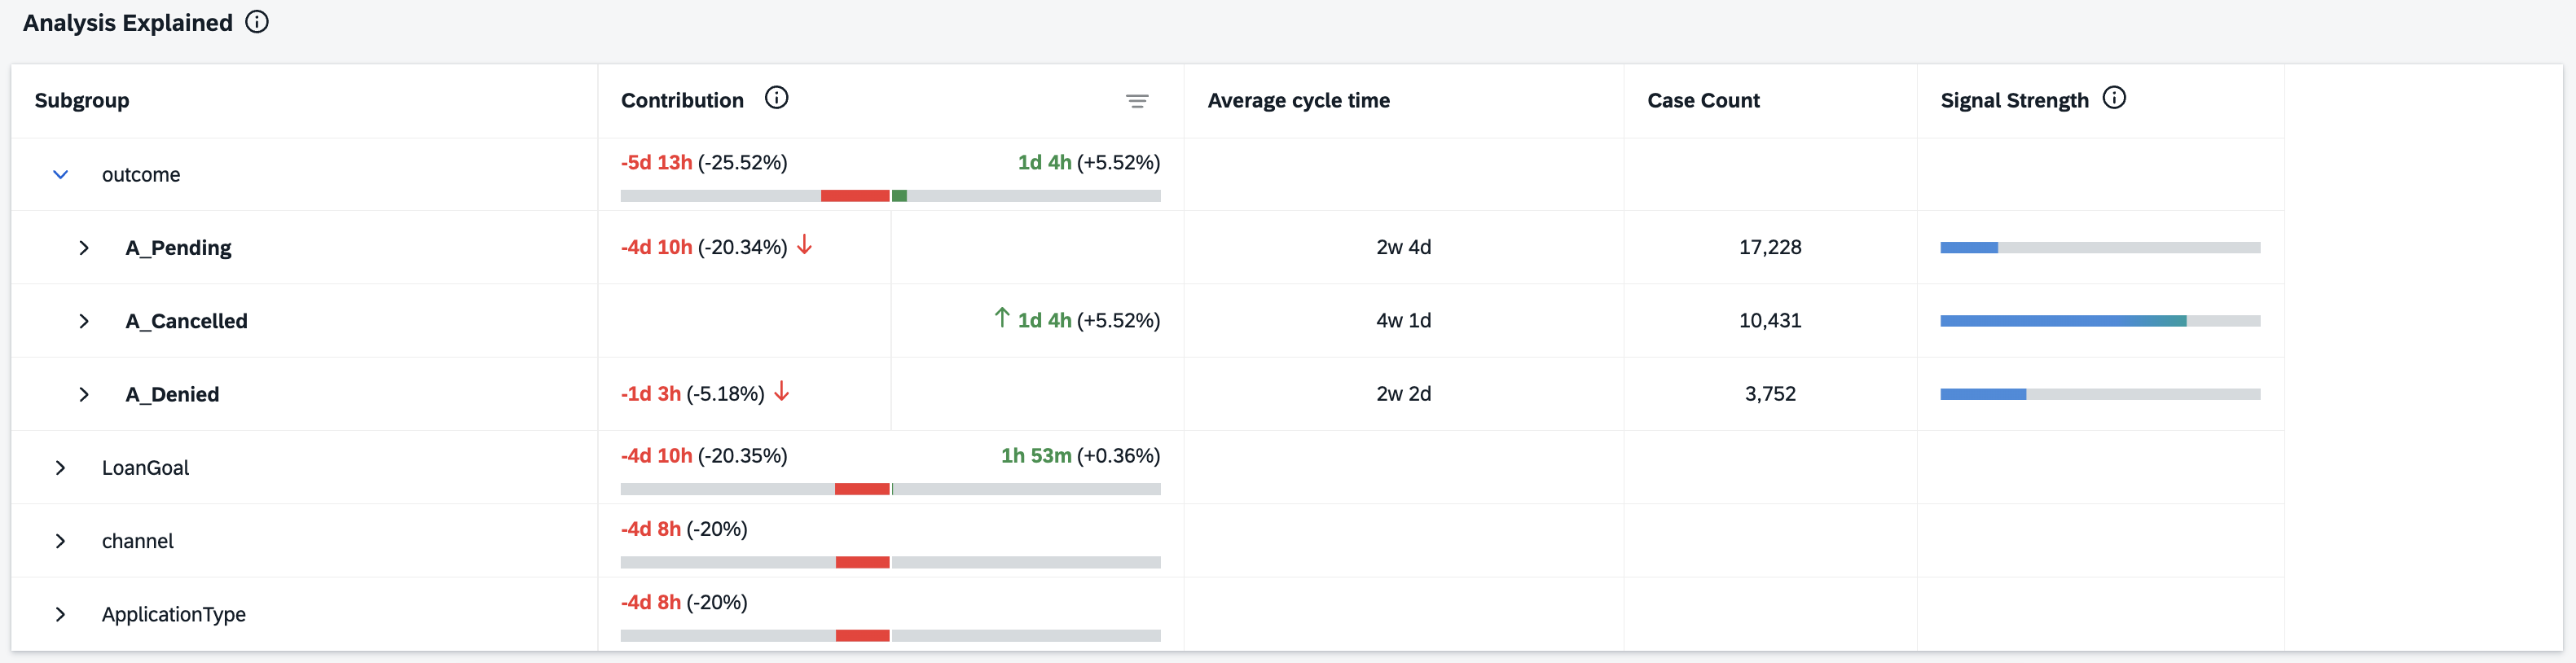
\includegraphics[width=\textwidth]{figures/Root_Cause_Analysis_1.png}\\[4pt]
  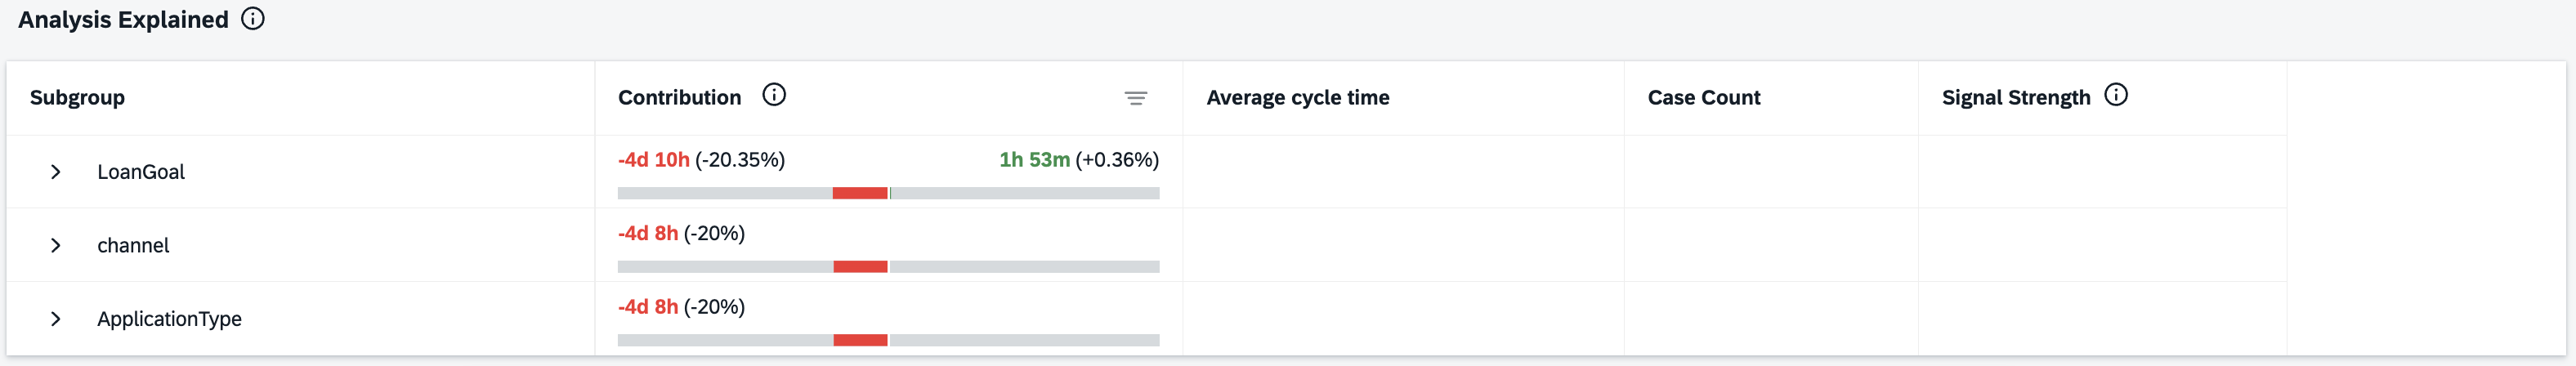
\includegraphics[width=\textwidth]{figures/Root_Cause_Analysis_2.png}
  \caption{Root cause analysis of the average cycle time with (top) and
  without (bottom) the outcome attribute.}
  \label{fig:sig_rca}
\end{figure}

\clearpage
\begin{figure}[h!]
  \centering
  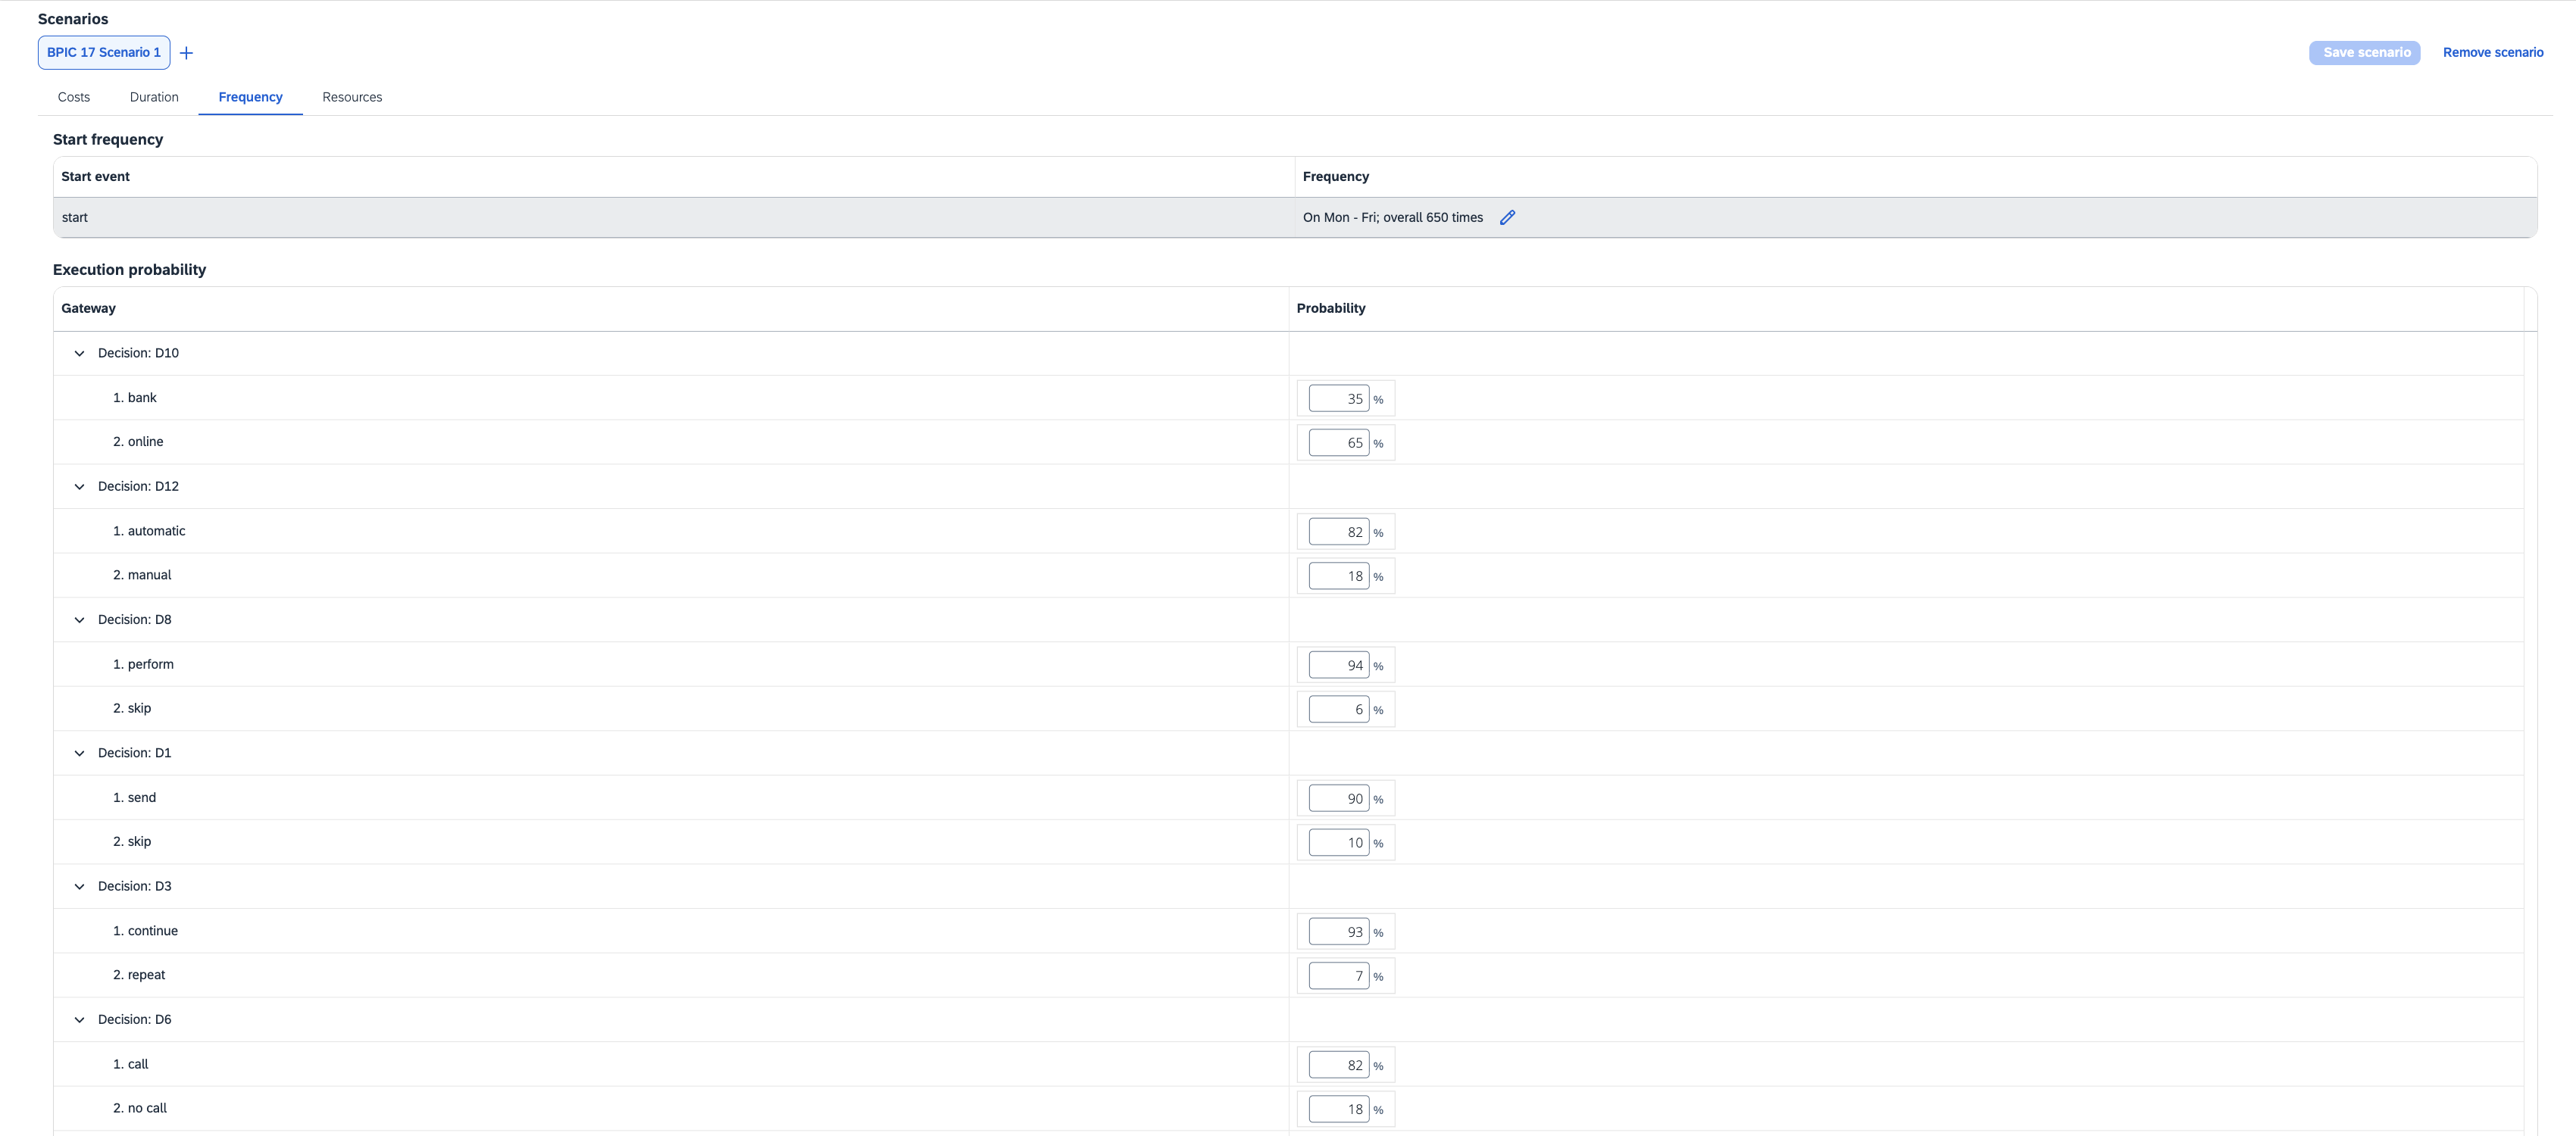
\includegraphics[width=0.8\textwidth]{figures/Simulation_list_1.png}\\[4pt]
  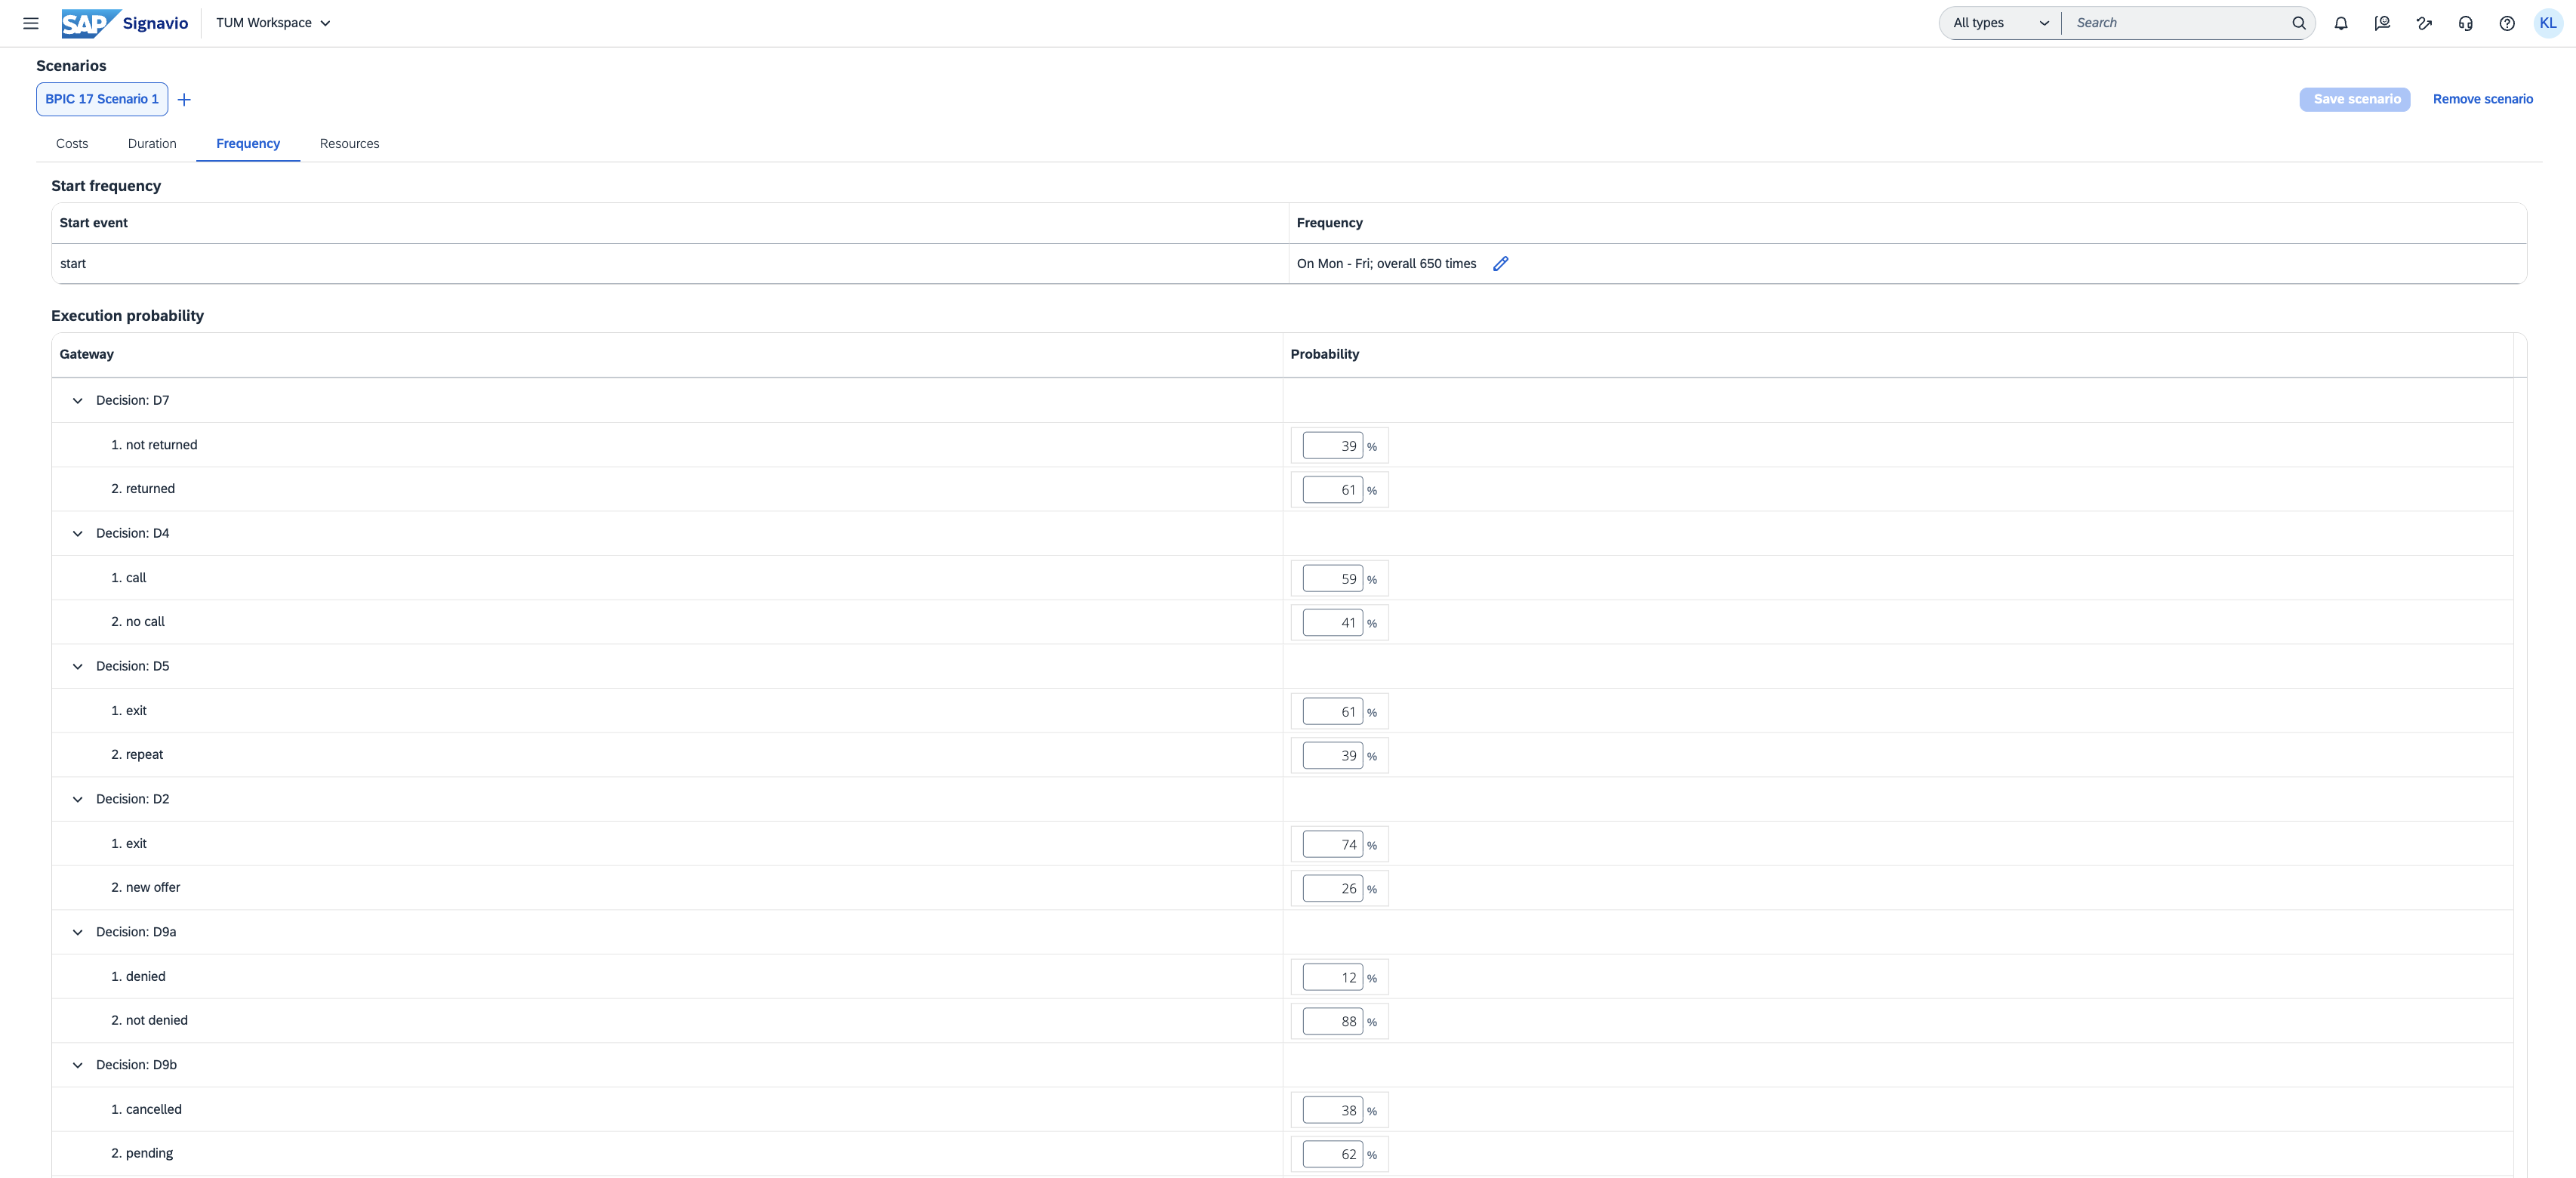
\includegraphics[width=0.8\textwidth]{figures/Simulation_list_2.png}\\[4pt]
  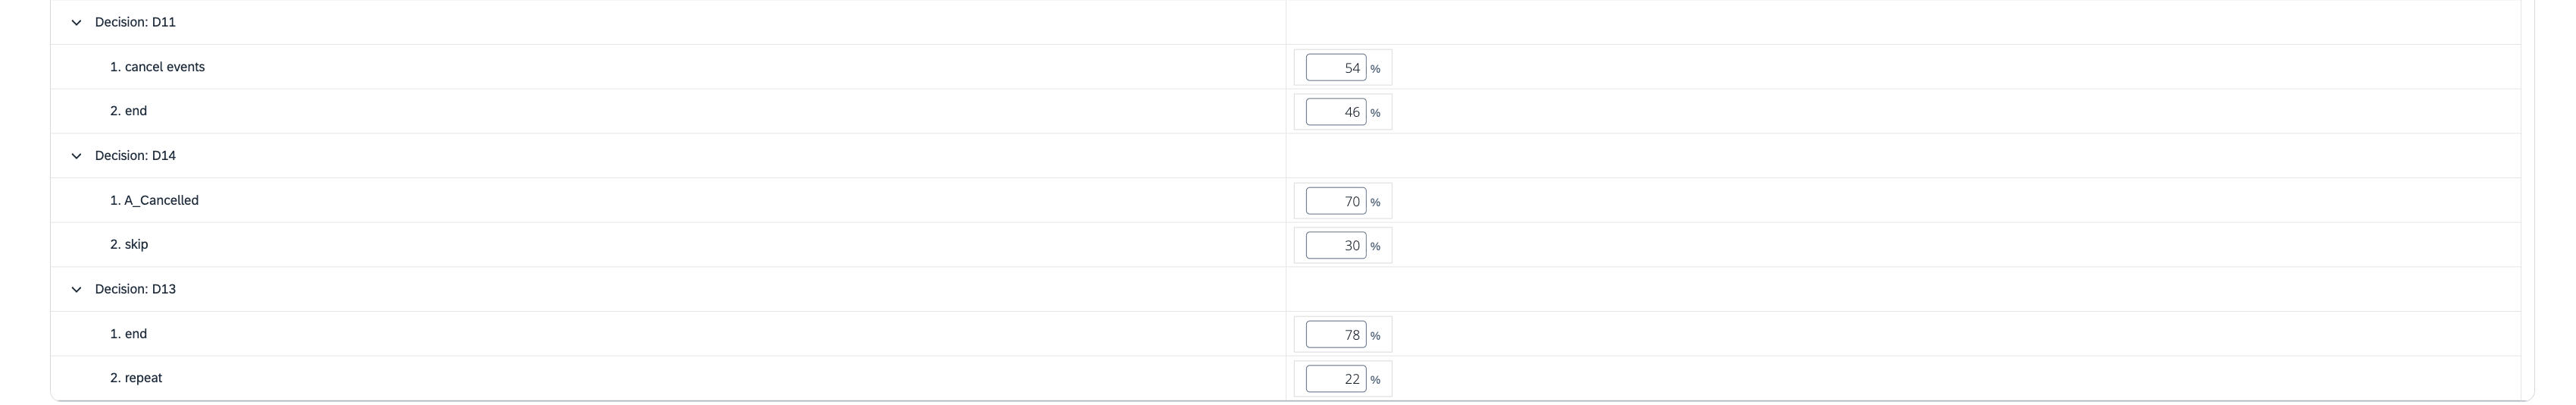
\includegraphics[width=0.8\textwidth]{figures/Simulation_list_3.png}
  \caption{Simulation scenario in Process Manager: start frequency and the
  branching probabilities of Table~\ref{tab:dpoints} at gateways D1--D14.}
  \label{fig:sig_scenario}
\end{figure}

\begin{figure}[h!]
  \centering
  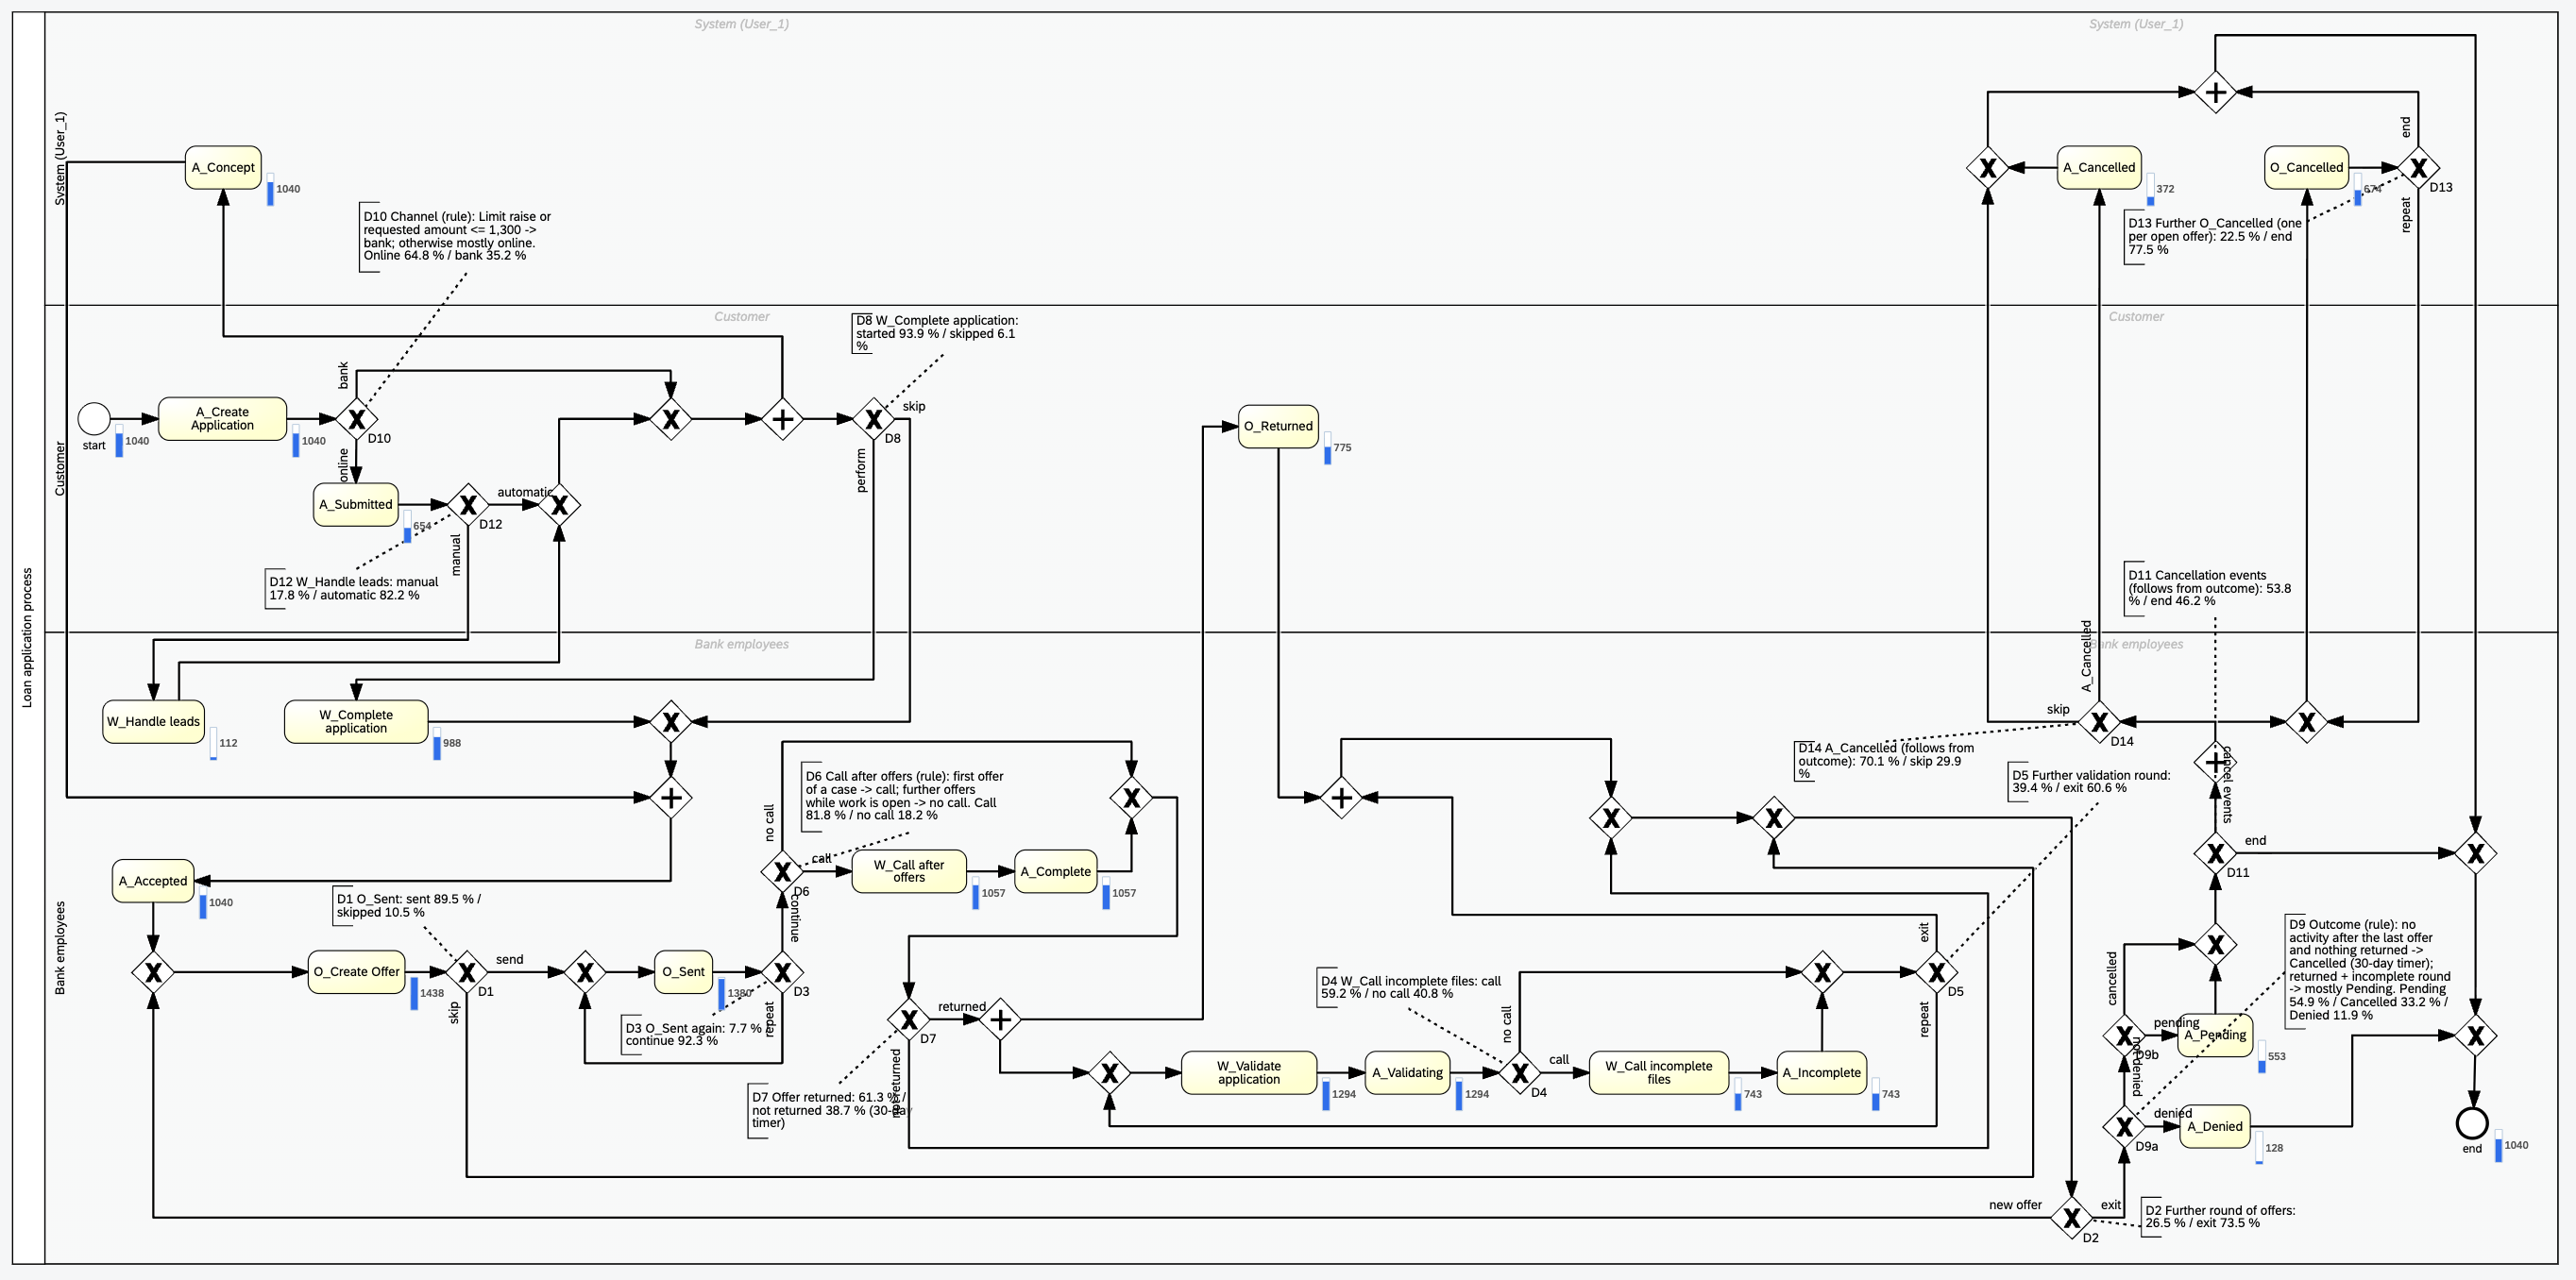
\includegraphics[width=\textwidth]{figures/Simulation_run_BPMN.png}
  \caption{Simulation run of 1,040 cases on the final BPMN; the bars show the
  number of completed instances per activity.}
  \label{fig:sig_run}
\end{figure}

\clearpage
\begin{figure}[h!]
  \centering
  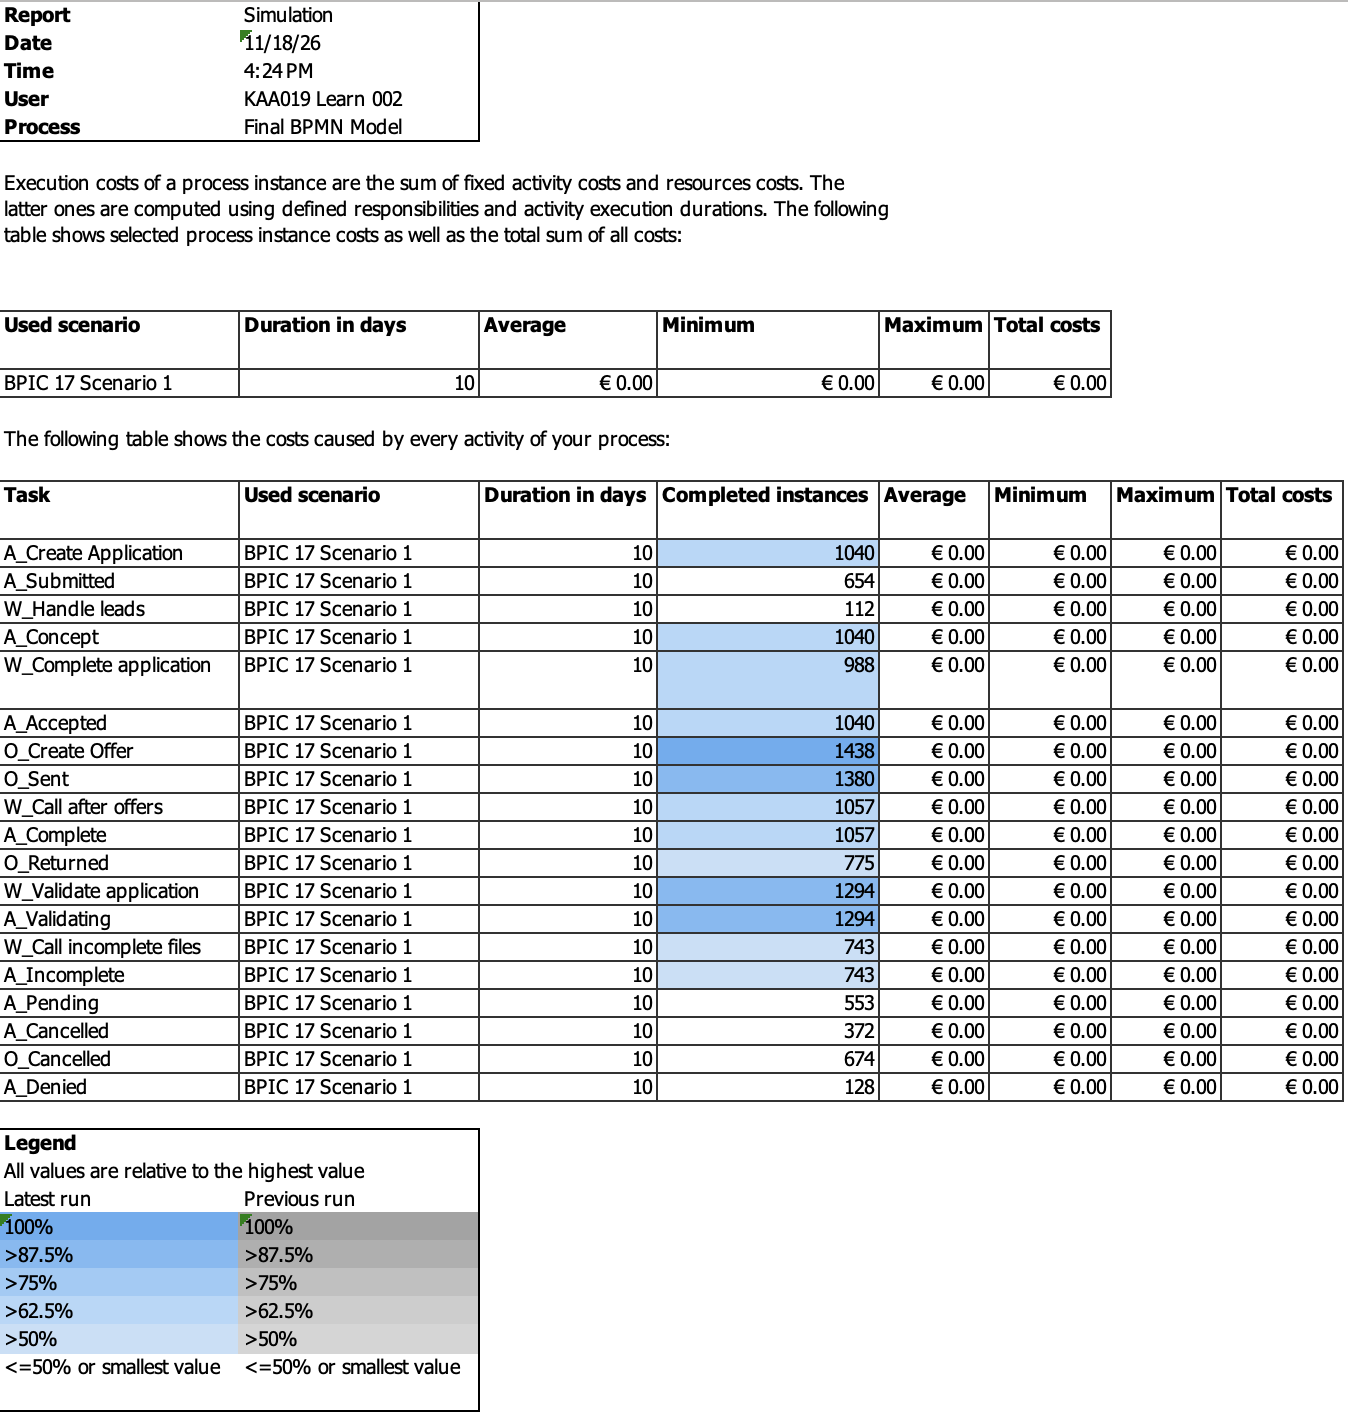
\includegraphics[width=0.65\textwidth]{figures/Signavio_simulation_results.png}
  \caption{Simulation report exported from SAP Signavio: completed instances
  per activity. The 553 + 372 + 128 = 1,053 end states exceed the 1,040
  simulated cases.}
  \label{fig:sig_report}
\end{figure}